% SampleProject.tex -- main LaTeX file for sample LaTeX article
%
%\documentclass[12pt]{article}
\documentclass[11pt]{SelfArxOneColBMN}
% add the pgf and tikz support.  This automatically loads
% xcolor so no need to load color
\usepackage{pgf}
\usepackage{tikz}
\usetikzlibrary{matrix}
\usetikzlibrary{calc}
\usepackage{xstring}
\usepackage{pbox}
\usepackage{etoolbox}
\usepackage{marginfix}
\usepackage{xparse}
\setlength{\parskip}{0pt}% fix as marginfix inserts a 1pt ghost parskip
% standard graphics support
\usepackage{graphicx,xcolor}
\usepackage{wrapfig}
%
\definecolor{color1}{RGB}{0,0,90} % Color of the article title and sections
\definecolor{color2}{RGB}{0,20,20} % Color of the boxes behind the abstract and headings
%----------------------------------------------------------------------------------------
% HYPERLINKS
%----------------------------------------------------------------------------------------
\usepackage[pdftex]{hyperref} % Required for hyperlinks
\hypersetup{hidelinks,
colorlinks,
breaklinks=true,%
urlcolor=color2,%
citecolor=color1,%
linkcolor=color1,%
bookmarksopen=false%
,pdftitle={FinalExam},%
pdfauthor={Peterson}}
%\usepackage[round,numbers]{natbib}
\usepackage[numbers]{natbib}
\usepackage{lmodern}
\usepackage{setspace}
\usepackage{xspace}
%
\usepackage{subfigure}
\newcommand{\goodgap}{
  \hspace{\subfigtopskip}
  \hspace{\subfigbottomskip}}
%
\usepackage{atbegshi}
%
\usepackage[hyper]{listings}
%
% use ams math packages
\usepackage{amsmath,amsthm,amssymb,amsfonts}
\usepackage{mathrsfs}
%
% use new improved Verbatim
\usepackage{fancyvrb}
%
\usepackage[titletoc,title]{appendix}
%
\usepackage{url}
%
% Create length for the baselineskip o text in footnotesize
\newdimen\footnotesizebaselineskip
\newcommand{\test}[1]{%
 \setbox0=\vbox{\footnotesize\strut Test \strut}
 \global\footnotesizebaselineskip=\ht0 \global\advance\footnotesizebaselineskip by \dp0
}
%
\usepackage{listings}

\DeclareGraphicsExtensions{.pdf, .jpg, .tif,.png}

% make sure we don't get orphaned words if at top of page
% or orphans if at bottom of page
\clubpenalty=9999
\widowpenalty=9999
\renewcommand{\textfraction}{0.15}
\renewcommand{\topfraction}{0.85}
\renewcommand{\bottomfraction}{0.85}
\renewcommand{\floatpagefraction}{0.66}
%
\DeclareMathOperator{\sech}{sech}

\newcommand{\mycite}[1]{%
(\citeauthor{#1} \citep{#1} \citeyear{#1})\xspace
}

\newcommand{\mycitetwo}[2]{%
(\citeauthor{#2} \citep[#1]{#2} \citeyear{#2})\xspace
}

\newcommand{\mycitethree}[3]{%
(\citeauthor{#3} \citep[#1][#2]{#3} \citeyear{#3})\xspace
}

\newcommand{\myincludegraphics}[3]{% file name, width, height
\includegraphics[width=#2,height=#3]{#1}
}

\newcommand{\myincludegraphicstwo}[2]{% file name, width, height
\includegraphics[scale=#1]{#2}
}

\newcommand{\mysimplegraphics}[1]{% file name, width, height
\includegraphics{#1}
}

\newcommand{\MB}[1]{
\boldsymbol{#1}
}

\newcommand{\myquotetwo}[1]{%
\small
%\singlespacing
\begin{quotation}
#1
\end{quotation}
\normalsize
%\onehalfspacing  
}

\newcommand{\jimquote}[1]{%
\small
%\singlespacing
\begin{quotation}
#1
\end{quotation}
\normalsize
%\onehalfspacing
}

\newcommand{\myquote}[1]{%
\small
%\singlespacing
\begin{quotation}
#1
\end{quotation}
\normalsize
%\onehalfspacing  
}

%A =
%
%[2 r_1 	     r_1]
%[-2r_1 + r_2  r_2 - r_1]
%
%has eigenvalues r_1 neq r_2.
% #1 = 2 r_1, #2 = r_1, #3 = -2r_1+r_2, #4 = r_2 - r_1
\newcommand{\myrealdiffA}[4]{
\left [
\begin{array}{rr}
#1  & #2\\
#3  & #4
\end{array}
\right ]
}

% args:
% 1, 2 ,3, 4, 5 = caption, label, width, height, file name
%\mysubfigure{}{}{}{}{}
\newcommand{\mysubfigure}[5]{%
\subfigure[#1]{\label{#2}\includegraphics[width=#3,height=#4]{#5}}
}

\newcommand{\mysubfiguretwo}[3]{%
\subfigure[#1]{\label{#2}\includegraphics{#3}}
}

\newcommand{\mysubfigurethree}[4]{%
\subfigure[#1]{\label{#2}\includegraphics[scale=#3]{#4}}
}

\newcommand{\myputimage}[5]{% file name, width, height
\centering
\includegraphics[width=#3,height=#4]{#5}
\caption{#1}
\label{#2}
}

\newcommand{\myputimagetwo}[4]{% caption, label, scale, file name
\centering
\includegraphics[scale=#3]{#4}
\caption{#1}
\label{#2}
}

\newcommand{\myrotateimage}[5]{% file name, width, height
\centering
\includegraphics[scale=#3,angle=#4]{#5}
\caption{#1}
\label{#2}
}

\newcommand{\myurl}[2]{%
\href{#1}{\bf #2}
}

\RecustomVerbatimEnvironment%
{Verbatim}{Verbatim}  
  {fillcolor=\color{black!20}}
  
  \DefineVerbatimEnvironment%
{MyVerbatim}{Verbatim}  
  {frame=single,
   framerule=2pt,
   fillcolor=\color{black!20},
   fontsize=\small}
   
\newcommand{\myfvset}[1]{%  
\fvset{frame=single,
       framerule=2pt,
       fontsize=\small,
       xleftmargin=#1in}}
       
\newcommand{\mylistverbatim}{%
\lstset{%
  fancyvrb, 
  basicstyle=\small,
  breaklines=true}
}  

\newcommand{\mylstinlinebf}[1]{%
{\bf #1}
}

\newcommand{\mylstinline}{%
\lstset{%
  basicstyle=\color{black!80}\bfseries\ttfamily,
  showstringspaces=false,
  showspaces=false,showtabs=false,
  breaklines=true}
\lstinline
}

\newcommand{\mylstinlinetwo}[1]{%
\lstset{%
  basicstyle=\color{black!80}\bfseries\ttfamily,
  showstringspaces=false,
  showspaces=false,showtabs=false,
  breaklines=true}
\lstinline!#1! 
}

%fontfamily=tt
%fontfamily=courier
%fontfamily=helvetica
%frame=topline,
%frame=single,
 %frame=lines,
 %framesep=10pt,
 %fontshape=it,
 %fontseries=b,
 %fontsize=\relsize{-1},
 %fillcolor=\color{black!20},
 %rulecolor=\color{yellow},
 %fillcolor=\color{red}
 %label=\fbox{\Large\emph{The code}}
\DefineVerbatimEnvironment%
{MyListVerbatim}{Verbatim}  
{
fillcolor=\color{black!10},
fontfamily=courier,
frame=single,
%formatcom=\color{white},
framesep=5mm,
labelposition=topline,
fontshape=it,
fontseries=b,
fontsize=\small,
label=\fbox{\large\emph{The code}\normalsize}
} 

%  caption={[#1] \large\bf{#1}}, 
%\centering \framebox[.6\textwidth][c]{\Large\bf{#1}}
\newcommand{\myfancyverbatim}[1]{%
\lstset{%
  fancyvrb=true, 
  %fvcmdparams= fillcolor 1,
  %morefvcmdparams = \textcolor 2,
  frame=shadowbox,framerule=2pt, 
  basicstyle=\small\bfseries,
  backgroundcolor=\color{black!08},
  showstringspaces=false,
  showspaces=false,showtabs=false,
  keywordstyle=\color{black}\bfseries,
  %numbers=left,numberstyle=\tiny,stepnumber=5,numbersep=5pt,
  stringstyle=\ttfamily,
  caption={[\quad #1] \mbox{}\\ \vspace{0.1in} \framebox{\large \bf{#1} \small} },  
  belowcaptionskip=20 pt,  
  label={},
  xleftmargin=17pt,
  framexleftmargin=17pt,
  framexrightmargin=5pt,
  framexbottommargin=4pt,
  nolol=false,
  breaklines=true}
}

\newcommand{\mylistcode}[3]{%
\lstset{%
  language=#1, 
  frame=shadowbox,framerule=2pt, 
  basicstyle=\small\bfseries,
  backgroundcolor=\color{black!16},
  showstringspaces=false,
  showspaces=false,showtabs=false,
  keywordstyle=\color{black!40}\bfseries,
  numbers=left,numberstyle=\tiny,stepnumber=5,numbersep=5pt,
  stringstyle=\ttfamily,
  caption={[\quad#2] \mbox{}\\ \vspace{0.1in} \framebox{\large \bf{#2} \small} },
  belowcaptionskip=20 pt,
  breaklines=true,
  xleftmargin=17pt,
  framexleftmargin=17pt,
  framexrightmargin=5pt,
  framexbottommargin=4pt,  
  label=#3,
  breaklines=true} 
}

  %caption={[#2] #3},
  %caption={[#2]{\mbox{}\\ \vspace{0.1in} \framebox{\large \bf{#3} \small}},
  %caption={[#2] \mbox{}\\ \bf{#3} },

% frame=single,
% caption={[Code Fragment] {\bf Code Fragment} },
% caption={[Code Fragment] \mbox{}\\ \vspace{0.1in} \framebox{\large \bf{Code Fragment} \small} },
\newcommand{\mylistcodequick}[1]{%
\lstset{%
  language=#1, 
  frame=shadowbox,framerule=2pt, 
  basicstyle=\small\bfseries,
  backgroundcolor=\color{black!16},
  showstringspaces=false,
  showspaces=false,showtabs=false,
  keywordstyle=\color{black!40}\bfseries,
  numbers=left,numberstyle=\tiny,stepnumber=5,numbersep=5pt,
  stringstyle=\ttfamily,
  caption={[\quad Code Fragment] \large \bf{Code Fragment} \small},   
  belowcaptionskip=20 pt,  
  label={},
  xleftmargin=17pt,
  framexleftmargin=17pt,
  framexrightmargin=5pt,
  framexbottommargin=4pt,
  breaklines=true} 
}

%  caption={[#2] \mbox{}\\ \vspace{0.1in} \framebox{\large \bf{#2} \small} },
\newcommand{\mylistcodequicktwo}[2]{%
\lstset{%
  language=#1, 
  frame=shadowbox,framerule=2pt, 
  basicstyle=\small\bfseries,
  extendedchars=true,
  backgroundcolor=\color{black!16},
  showstringspaces=false,
  showspaces=false,
  showtabs=false,
  keywordstyle=\color{black!40}\bfseries,
  numbers=left,numberstyle=\tiny,stepnumber=5,numbersep=5pt,
  stringstyle=\ttfamily,
  caption={[\quad#2] \large \bf{#2} \small},
  belowcaptionskip=20 pt,
  label={},
  xleftmargin=17pt,
  framexleftmargin=17pt,
  framexrightmargin=5pt,
  framexbottommargin=4pt,
  breaklines=true} 
}

%  caption={[#2] \mbox{}\\ \vspace{0.1in} \framebox{\large \bf{#2} \small} },
\newcommand{\mylistcodequickthree}[2]{%
\lstset{%
  language=#1, 
  frame=shadowbox,framerule=2pt, 
  basicstyle=\small\bfseries,
  extendedchars=true,
  backgroundcolor=\color{black!16},
  showstringspaces=false,
  showspaces=false,
  showtabs=false,
  keywordstyle=\color{black!40}\bfseries,
  numbers=left,numberstyle=\tiny,stepnumber=5,numbersep=5pt,
  stringstyle=\ttfamily,
  caption={[\quad#2] \large\bf{#2}\small},
  belowcaptionskip=20 pt,
  label={},
  xleftmargin=17pt,
  framexleftmargin=17pt,
  framexrightmargin=5pt,
  framexbottommargin=4pt,
  breaklines=true} 
}

%  frame=single,
\newcommand{\mylistset}[4]{%
\lstset{language=#1,
  basicstyle=\small,
  showstringspaces=false,
  showspaces=false,showtabs=false,
  keywordstyle=\color{black!40}\bfseries,
  numbers=left,numberstyle=\tiny,stepnumber=5,numbersep=5pt,
  stringstyle=\ttfamily,
  caption={[\quad#2]#3},
  label=#4}
}

\newcommand{\mylstinlineset}{%
\lstset{%
  basicstyle=\color{blue}\bfseries\ttfamily,
  showstringspaces=false,
  showspaces=false,showtabs=false,
  breaklines=true}
}

\newcommand{\myframedtext}[1]{%
\centering
\noindent
%\fbox{\parbox[c]{.9\textwidth}{\color{black!40} \small \singlespacing #1\onehalfspacing \normalsize \\}}
\fbox{\parbox[c]{.9\textwidth}{\color{black!40} \small  #1 \normalsize \\}}
}

\newcommand{\myemptybox}[2]{% from , to
\fbox{\begin{minipage}[t][#1in][c]{#2in}\hspace{#2in}\end{minipage}}
}

\newcommand{\myemptyboxtwo}[2]{% from , to
\centering\fbox{
\begin{minipage}{#1in}
\hfill\vspace{#2in}
\end{minipage}
}
}

\newcommand{\boldvector}[1]{
\boldsymbol{#1}
}

\newcommand{\dEdY}[2]{\frac{d E}{d Y_{#1}^{#2}}}
\newcommand{\dEdy}[2]{\frac{d E}{d y_{#1}^{#2}}}
\newcommand{\dEdT}[2]{\frac{\partial E}{\partial T_{{#1} \rightarrow {#2}}}}
\newcommand{\dEdo}[1]{\frac{\partial E}{\partial o^{#1}}}
\newcommand{\dEdg}[1]{\frac{\partial E}{\partial g^{#1}}}
\newcommand{\dYdY}[4]{\frac{\partial Y_{#1}^{#2}}{\partial Y_{#3}^{#4}}}
\newcommand{\dYdy}[4]{\frac{\partial Y_{#1}^{#2}}{\partial y_{#3}^{#4}}}
\newcommand{\dydY}[4]{\frac{\partial y_{#1}^{#2}}{\partial Y_{#3}^{#4}}}
\newcommand{\dydy}[4]{\frac{\partial y_{#1}^{#2}}{\partial y_{#3}^{#4}}}
\newcommand{\dydT}[4]{\frac{\partial y_{#1}^{#2}}{\partial T_{{#3} \rightarrow {#4}}}}
\newcommand{\dYdT}[4]{\frac{\partial Y_{#1}^{#2}}{\partial T_{{#3} \rightarrow {#4}}}}
\newcommand{\dTdT}[4]{\frac{\partial T_{{#1} \rightarrow {#2}}}{\partial T_{{#3} \rightarrow {#4}}}}
\newcommand{\ssum}[2]{\sum_{#1}^{#2}}

\newcommand{\ssty}[1]{\scriptscriptstyle #1}

\newcommand{\myparbox}[2]{%
\parbox{#1}{\color{black!20} #2}
}

\newcommand{\bs}[1]{
\boldsymbol{#1}
}

\newcommand{\parone}[2]{%
\frac{\partial #1 }{ \partial #2 }
}
\newcommand{\partwo}[2]{%
\frac{ \partial^2 {#1} }{ \partial {#2}^2 }
}

\newcommand{\twodvectorvarfun}[2]{
\left [
\begin{array}{r}
{{#1_{\ssty{1}}}(#2)} \\
{{#1_{\ssty{2}}}(#2)}
\end{array}
\right ]
}
\newcommand{\twodvectorvarprimed}[1]{
\left [
\begin{array}{r}
{{#1_{\ssty{1}}}'(t)} \\
{{#1_{\ssty{2}}}'(t)}
\end{array}
\right ]
}

\newcommand{\complex}[2]{#1 \: #2 \: \boldsymbol{i}}
\newcommand{\complexmag}[2]%
{
\sqrt{(#1)^2 \: + \: (#2)^2}
}
\newcommand{\threenorm}[3]%
{
\sqrt{(#1)^2 \: + \: (#2)^2 \: + \: (#3)^2}
}
\newcommand{\norm}[1]{\mid \mid #1 \mid \mid}

\newcommand{\myderiv}[2]{\frac{d #1}{d #2}}
\newcommand{\myderivb}[2]{\frac{d}{d #2} \left ( #1 \right )}
\newcommand{\myrate}[3]%
{#1^\prime(#2) &=& #3 \: #1(#2)
}
\newcommand{\myrateexter}[4]%
{#1^\prime(#2) &=& #3 \: #1(#2) \: + \: #4
}
\newcommand{\myrateic}[3]%
{#1( \: #2 \:) &=& #3 
}

\newcommand{\mytwodsystemeqn}[6]{
#1 \: x    #2 \: y &=& #3\\
#4 \: x    #5 \: y &=& #6\\
}

\newcommand{\mytwodsystem}[8]{
#3 \: #1 \: + \: #4 \: #2 &=& #5\\
#6 \: #1 \: + \: #7 \: #2 &=& #8\\
}  

\newcommand{\mytwodarray}[4]{
\left [
\begin{array}{rr}
#1 & #2\\
#3 & #4
\end{array}
\right ]
}

\newcommand{\mytwoid}{
\left [
\begin{array}{rr}
1 & 0\\
0 & 1
\end{array}
\right ]
}

\newcommand{\myxprime}[2]{
\left [
\begin{array}{r}
#1^\prime(t)\\
#2^\prime(t)
\end{array}
\right ]
}

\newcommand{\myxprimepacked}[2]{
\left [
\begin{array}{r}
#1^\prime\\
#2^\prime
\end{array}
\right ]
}

\newcommand{\myx}[2]{
\left [
\begin{array}{r}
#1(t)\\
#2(t)
\end{array}
\right ]
}

\newcommand{\myxonly}[2]{
\left [
\begin{array}{r}
#1\\
#2
\end{array}
\right ]
}

\newcommand{\myv}[2]{
\left [
\begin{array}{r}
#1\\
#2
\end{array}
\right ]
}

\newcommand{\myxinitial}[2]{
\left [
\begin{array}{r}
#1(0)\\
#2(0)
\end{array}
\right ]
}

\newcommand{\twodboldv}[1]{
\boldsymbol{#1}
}

\newcommand{\mytwodvector}[2]{
\left [
\begin{array}{r}
#1\\
#2
\end{array}
\right ]
}

\newcommand{\mythreedvector}[3]{
\left [
\begin{array}{r}
#1\\
#2\\
#3
\end{array}
\right ]
}

\newcommand{\mytwodsystemvector}[6]{
\left [
\begin{array}{rr}
#1 & #2\\
#4 & #5
\end{array}
\right ]
\:
\left [
\begin{array}{r}
x \\
y 
\end{array}
\right ]
&=&
\left [
\begin{array}{r}
#3\\
#6
\end{array}
\right ]
}

\newcommand{\mythreedarray}[9]{
\left [
\begin{array}{rrr}
#1 & #2 & #3\\
#4 & #5 & #6\\
#7 & #8 & #9
\end{array}
\right ]
}

\newcommand{\myodetwo}[6]{
#1 \: #6^{\prime \prime}(t) \: #2 \: #6^{\prime}(t) \: #3 \: #6(t) &=& 0\\
#6(0)                                           &=& #4\\
#6^{\prime}(0)                                  &=& #5
}

\newcommand{\myodetwoNoIC}[4]{
#1 \: #4^{\prime \prime}(t) \: #2 \: #4^{\prime}(t) \: #3 \: #4(t) &=& 0
}

\newcommand{\myodetwopacked}[5]{
\hspace{-0.3in}& & #1 u^{\prime \prime} #2 u^{\prime} #3 u \: = \: 0\\
\hspace{-0.3in}& & u(0) \: = \: #4, \: \: u^{\prime}(0)    \: = \:  #5
}

\newcommand{\myodetwoforced}[6]{
#1\: u^{\prime \prime}(t) \: #2 \: u^{\prime}(t) \: #3 \: u(t) &=& #6\\
u(0)                                           &=& #4\\
u^{\prime}(0)                                  &=& #5\\
}

\newcommand{\myodesystemtwo}[8]{
#1 \: x^\prime(t) \: #2 \: y^\prime(t) \: #3 \: x(t) \: #4 \: y(t) &=& 0\\
#5 \: x^\prime(t) \: #6 \: y^\prime(t) \: #7 \: x(t) \: #8 \: y(t) &=& 0\\
}

\newcommand{\myodesystemtwoic}[2]{
x(0)                                       &=& #1\\ 
y(0)                                       &=& #2
}

\newcommand{\mypredprey}[4]{
x^\prime(t) &=& #1 \: x(t) \: - \: #2 \: x(t) \: y(t)\\
y^\prime(t) &=& -#3 \: y(t) \: + \: #4 \: x(t) \: y(t)
}

\newcommand{\mypredpreypacked}[4]{
x^\prime &=& #1 \: x - #2 \: x \: y\\
y^\prime &=& -#3 \: y + #4 \: x \: y
}

\newcommand{\mypredpreyself}[6]{
x^\prime(t) &=&  #1 \: x(t) \: - \: #2 \: x(t) \: y(t) \: - \: #3 \: x(t)^2\\
y^\prime(t) &=& -#4 \: y(t) \: + \: #5 \: x(t) \: y(t) \: - \: #6 \: y(t)^2
}

\newcommand{\mypredpreyfish}[5]{
x^\prime(t) &=&  #1 \: x(t) \: - \: #2 \: x(t) \: y(t) \: - \: #5 \: x(t)\\
y^\prime(t) &=& -#3 \: y(t) \: + \: #4 \: x(t) \: y(t) \: - \: #5 \: y(t)
}

\newcommand{\myepidemic}[4]{
S^\prime(t) &=& - #1 \: S(t) \: I(t)\\
I^\prime(t) &=&   #1 \: S(t) \: I(t) \: - \: #2 \: I(t)\\
S(0)        &=&   #3\\
I(0)        &=&   #4\\
}

\newcommand{\bsred}[1]{%
\textcolor{red}{\boldsymbol{#1}}
}

\newcommand{\bsblue}[1]{%
\textcolor{blue}{\boldsymbol{#1}}
}


\newcommand{\myfloor}[1]{%
\lfloor{#1}\rfloor
}

\newcommand{\cubeface}[7]{%
\begin{bmatrix}
\bs{#3}          & \longrightarrow & \bs{#4}\\
\uparrow          &                         &  \uparrow  \\
\bs{#1} & \longrightarrow & \bs{#2}\\
              & \text{ \bfseries #5:} \: \bs{#6} \: \text{\bfseries  #7 } & 
\end{bmatrix}
}

\newcommand{\cubefacetwo}[5]{%
\begin{bmatrix}
\bs{#3}          & \longrightarrow & \bs{#4}\\
\uparrow          &                         &  \uparrow  \\
\bs{#1} & \longrightarrow & \bs{#2}\\
              & \text{ \bfseries #5} & 
\end{bmatrix}
}

\newcommand{\cubefacethree}[9]{%
\begin{bmatrix}
\bs{#3}                  & \overset{#9}{\longrightarrow} & \bs{#4}\\
\uparrow \: #7         &                                             &  \uparrow  \: #8 \\
\bs{#1}                  & \overset{#6}{\longrightarrow} & \bs{#2}\\
                               & \text{ \bfseries #5} & 
\end{bmatrix}
}

\renewcommand{\qedsymbol}{\hfill \blacksquare}
\newcommand{\subqedsymbol}{\hfill \Box}
%\theoremstyle{plain}

\newtheoremstyle{mystyle}% name
  {6pt}%      Space above
  {6pt}%      Space below
  {\itshape}%         Body font
  {}%         Indent amount (empty = no indent, \parindent = para indent)
  {\bfseries}% Thm head font
  {}%        Punctuation after thm head
  { }%     Space after thm head: " " = normal interword space; \newline = linebreak
  {}%         Thm head spec (can be left empty, meaning `normal')
\theoremstyle{mystyle}
 
\newtheorem{axiom}{Axiom}
%\newtheorem{solution}{Solution}[section]
\newtheorem*{solution}{Solution}
\newtheorem{exercise}{Exercise}[section]
\newtheorem{theorem}{Theorem}[section]
\newtheorem{proposition}[theorem]{Proposition}
\newtheorem{prop}[theorem]{Proposition}
\newtheorem{assumption}{Assumption}[section]
\newtheorem{definition}{Definition}[section]
\newtheorem{comment}{Comment}[section]
\newtheorem*{question}{Question}
\newtheorem{program}{Program}[section]
%\newtheorem{myproof}{Proof}
%\newtheorem*{myproof}{Proof}[section]
\newtheorem{myproof}{Proof}[section]
\newtheorem{hint}{Hint}[section]
\newtheorem*{phint}{Hint}
\newtheorem{lemma}[theorem]{Lemma}
\newtheorem{example}{Example}[section]
      
\newenvironment{myassumption}[4]
{
\centering
\begin{assumption}[{\textbf{#1}\nopunct}]%
\index{#2}
\mbox{}\\  \vskip6pt \colorbox{black!15}{\fbox{\parbox{.9\textwidth}{#3}}}
\label{#4}
\end{assumption}
%\renewcommand{\theproposition}{\arabic{chapter}.\arabic{section}.\arabic{assumption}} 
}%
{}

\newenvironment{myproposition}[4]
{
\centering
\begin{proposition}[{\textbf{#1}\nopunct}]%
\index{#2} 
\mbox{}\\  \vskip6pt \colorbox{black!15}{\fbox{\parbox{.9\textwidth}{#3}}}
\label{#4}
\end{proposition}
%\renewcommand{\theproposition}{\arabic{chapter}.\arabic{section}.\arabic{proposition}} 
}%
{}

\newenvironment{mytheorem}[4]
{
\centering
\begin{theorem}[{\textbf{#1}\nopunct}]%
\index{#2} 
\mbox{}\\ \vskip6pt \colorbox{black!15}{\fbox{\parbox{.9\textwidth}{#3}}}
\label{#4}
\end{theorem}
%\renewcommand{\thetheorem}{\arabic{chapter}.\arabic{section}.\arabic{theorem}} 
}%
{}

\newenvironment{mydefinition}[4]
{
\centering
\begin{definition}[{\textbf{#1}\nopunct}]%
\index{#2} 
\mbox{}\\  \vskip6pt \colorbox{black!15}{\fbox{\parbox{.9\textwidth}{#3}}}
\label{#4}
\end{definition}
%\renewcommand{\thedefinitio{n}{\arabic{chapter}.\arabic{section}.\arabic{definition}} 
}%
{}

\newenvironment{myaxiom}[4]
{
\centering
\begin{axiom}[{\textbf{#1}\nopunct}]%
\index{#2} 
\mbox{}\\  \vskip6pt \colorbox{black!15}{\fbox{\parbox{.9\textwidth}{#3}}}
\label{#4}
\end{axiom}
%\renewcommand{\theaxiom}{\arabic{chapter}.\arabic{section}.\arabic{axiom}} 
}%
{}

\newenvironment{mylemma}[4]
{
\centering
\begin{lemma}[{\textbf{#1}\nopunct}]%
\index{#2} 
\mbox{}\\  \vskip6pt \colorbox{black!15}{\fbox{\parbox{.9\textwidth}{#3}}}
\label{#4}
\end{lemma}
%\renewcommand{\thelemma}{\arabic{chapter}.\arabic{section}.\arabic{lemma}} 
}%
{}
   
\newenvironment{reason}[1]
{
 \vskip0.05in
 \begin{myproof}
 \mbox{}\\#1
 $\qedsymbol$
 \end{myproof}  
 \vskip0.05in
}%
{}

\newenvironment{reasontwo}[1]
{
 \vskip+.05in
 \begin{myproof}
 \mbox{}\\#1
 \end{myproof}  
 \vskip+0.05in
}%
{}

\newenvironment{subreason}[1]
{
 \vskip0.05in
 \renewcommand{\themyproof}{}
 \begin{myproof}
 #1
 $\subqedsymbol$
 \end{myproof}
 \vskip0.05in
 \renewcommand{\themyproof}{\thetheorem}
 %\renewcommand{\themyproof}{\arabic{chapter}.\arabic{section}.\arabic{myproof}}   
 %
}%
{}  

\newenvironment{myhint}[1]
{
 \vskip0.05in
 \begin{hint}
 #1
 $\subqedsymbol$ 
 \end{hint}  
 \vskip0.05in
}%
{} 

\newenvironment{myeqn}[3]
{
 \renewcommand{\theequation}{$\boldsymbol{#1}$}
 \begin{eqnarray}
 \label{equation:#2}
 #3 
 \end{eqnarray}
 \renewcommand{\theequation}{\arabic{chapter}.\arabic{eqnarray}}   
}%
{} 


\JournalInfo{Econ 8050:  Final Exam, 1-\pageref{LastPage}, 2020} % Journal information
\Archive{Draft Version \today} % Additional notes (e.g. copyright, DOI, review/research article)

\PaperTitle{Econ 8050 Final Exam}
\Authors{Ian Davis\textsuperscript{1}}
\affiliation{\textsuperscript{1}\textit{John E. Walker Department of Economics,
Clemson University,Clemson, SC: email ijdavis@g.clemson.edu}}
%\affiliation{*\textbf{Corresponding author}: yournamehere@clemson.edu} % Corresponding author

\date{\small{Version ~\today}}
\Abstract{Questions from Final Exam}
\Keywords{None}
\newcommand{\keywordname}{Keywords}
%
\onehalfspacing
\begin{document}

\flushbottom

\addcontentsline{toc}{section}{Title}
\maketitle

\renewcommand{\theexercise}{\arabic{exercise}}%

\begin{enumerate}
  \item Consider a Solow model with both physical $(K)$ and human $(H)$ capital. The production functions is given by
  \begin{eqnarray*}
    Y_t = K_t^\alpha H_t^\beta L_t^{1 - \alpha - \beta}
  \end{eqnarray*}
  where $\alpha + \beta < 1$. The number of workers grows over time at an exogenous and constatnt rate $n$ according to
  \begin{eqnarray*}
    L_{t+1} = (1 + n)L_t
  \end{eqnarray*}
  Assume that a constant fraction of output $s_K$ $(s_H)$ is invested in physical (human) capital. Physical capital depreciates at the rate of $\delta$ but human capital does not depreciate at all.
  \begin{enumerate}
    \item Derive the equations of the phase diagram showing the dynamics of the model. Explain what variables you are using for your analysis.
    \begin{solution}
      First, we want to normalize $A = 1$ for simplicity of notation and we can do this because of its constant nature. Next, we need to address the ramifications of Labor constantly growing. The growth of Labor will force us to use the variables \textbf{Human Capital per Capita} and \textbf{Physical Capital per Capita} in our phase diagram as opposed to the usual aggregate values. Let's first note the behavior of $H_t$ and $K_t$
      \begin{eqnarray*}
        K_{t+1} - K_t &=& s_KK_t^\alpha H_t^\beta L^{1 - \alpha - \beta} - \delta K_t\\
        H_{t+1} - H_t &=& s_HK_t^\alpha H_t^\beta L^{1 - \alpha - \beta}
      \end{eqnarray*}
      Setting $\Delta K = 0$ we find
      \begin{eqnarray*}
        s_KH_t^\beta L^{1 - \alpha - \beta} &=& \delta K\\
        \implies (\frac{s_K}{\delta})H_t^\beta L^{1 - \alpha - \beta} &=& K^{1 - \alpha}\\
        \implies (\frac{s_K}{\delta})^\frac{1}{1 - \alpha}H_t^\frac{\beta}{1 - \alpha} L^\frac{1 - \alpha - \beta}{1 - \alpha} &=& K^*
      \end{eqnarray*}
      and dividing both sides by $L_t$ to give us per worker values leaves us with
      \begin{eqnarray*}
        (\frac{s_K}{\delta + n})^\frac{1}{1 - \alpha}h_t^\frac{\beta}{1 - \alpha} = k
      \end{eqnarray*}
      where $k$ is constant. In similar fashion, we can substitute values in values of $H_t$ to find a constant $h$ as
      \begin{eqnarray*}
        (\frac{s_H}{n})^\frac{1}{1 - \beta}k_t^\frac{\alpha}{1 - \beta} = h
      \end{eqnarray*}
    \end{solution}
    \item Draw that phase diagram showing the dynamics of the model and the steady state. make sure you show the arrows indicating the dynamics of the steady state.
    \begin{solution}
    \end{solution}
      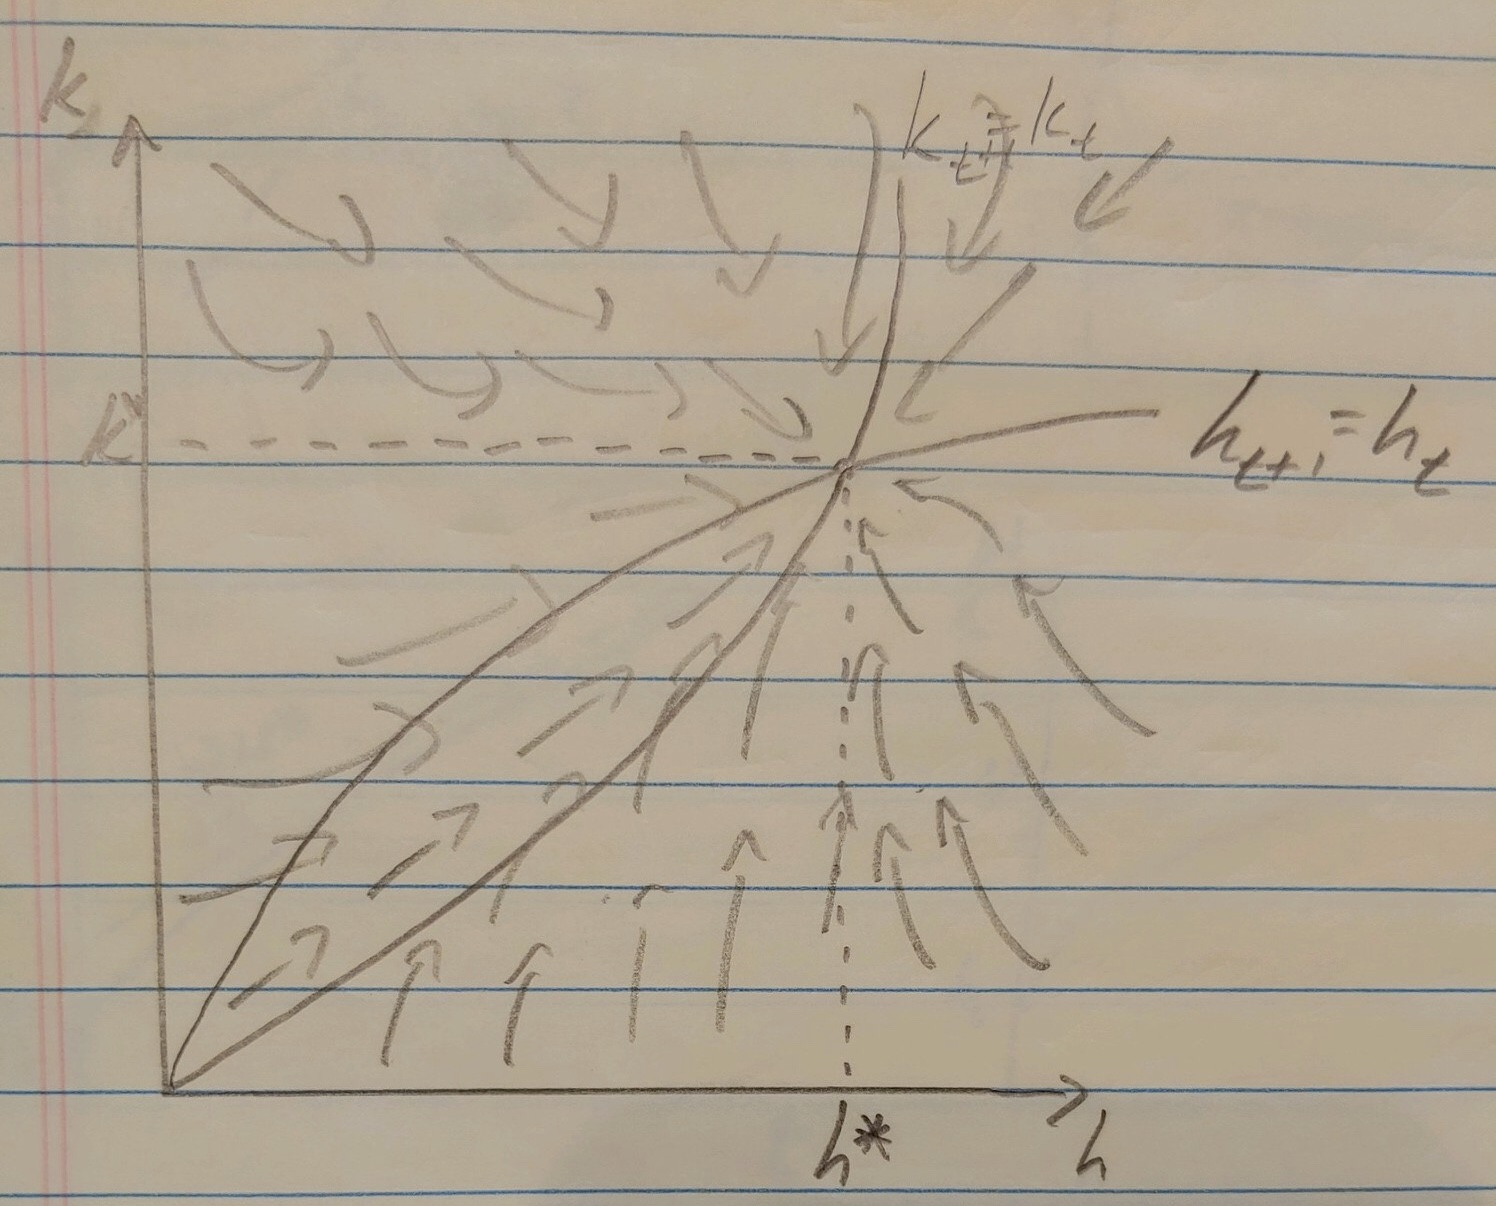
\includegraphics[scale=.185]{graph1b.JPG}\\
      \centering
    \item In steady state, what will be the growth rate of per worker values $(\frac{Y}{L},\frac{H}{L},\frac{K}{L})$? How about total $GDP$, $H$, and $K$? Explain your answers.
    \begin{solution}
      In the steady state, the growth rate of each of the per worker values will be zero but the aggregate values of GDP, H, and K will continue to grow because Labor continues to grow. This is because the growth of each of these aggregate values reaches a steady state which is equivalent to the growth of Labor. Hence, in all of the per worker values, the growth of the numerator is cancled by the growth of the denominator and we are left with an unchanging value as $t$ increases.
      
    \end{solution}
    \item Show how an economy that starts with a low level of human capital and physical capital will get to the steady state. Use the phase diagram as well as time-series plots of $K$ and $H$.
    \begin{solution}
      As shown in the graphs below, the phase diagram shows the economy starting at $(k_0,h_0)$ will eventually move to the steady state values of $(k^*,h^*)$ but the time series plots of $H_t$ and $K_t$ only converge to a steady state value of $\frac{\partial K}{\partial t}$ and $\frac{\partial H}{\partial t}$. The time plots of $\frac{K}{L} = k$ and $\frac{H}{L} = H$ do reach steady state values however.\\
      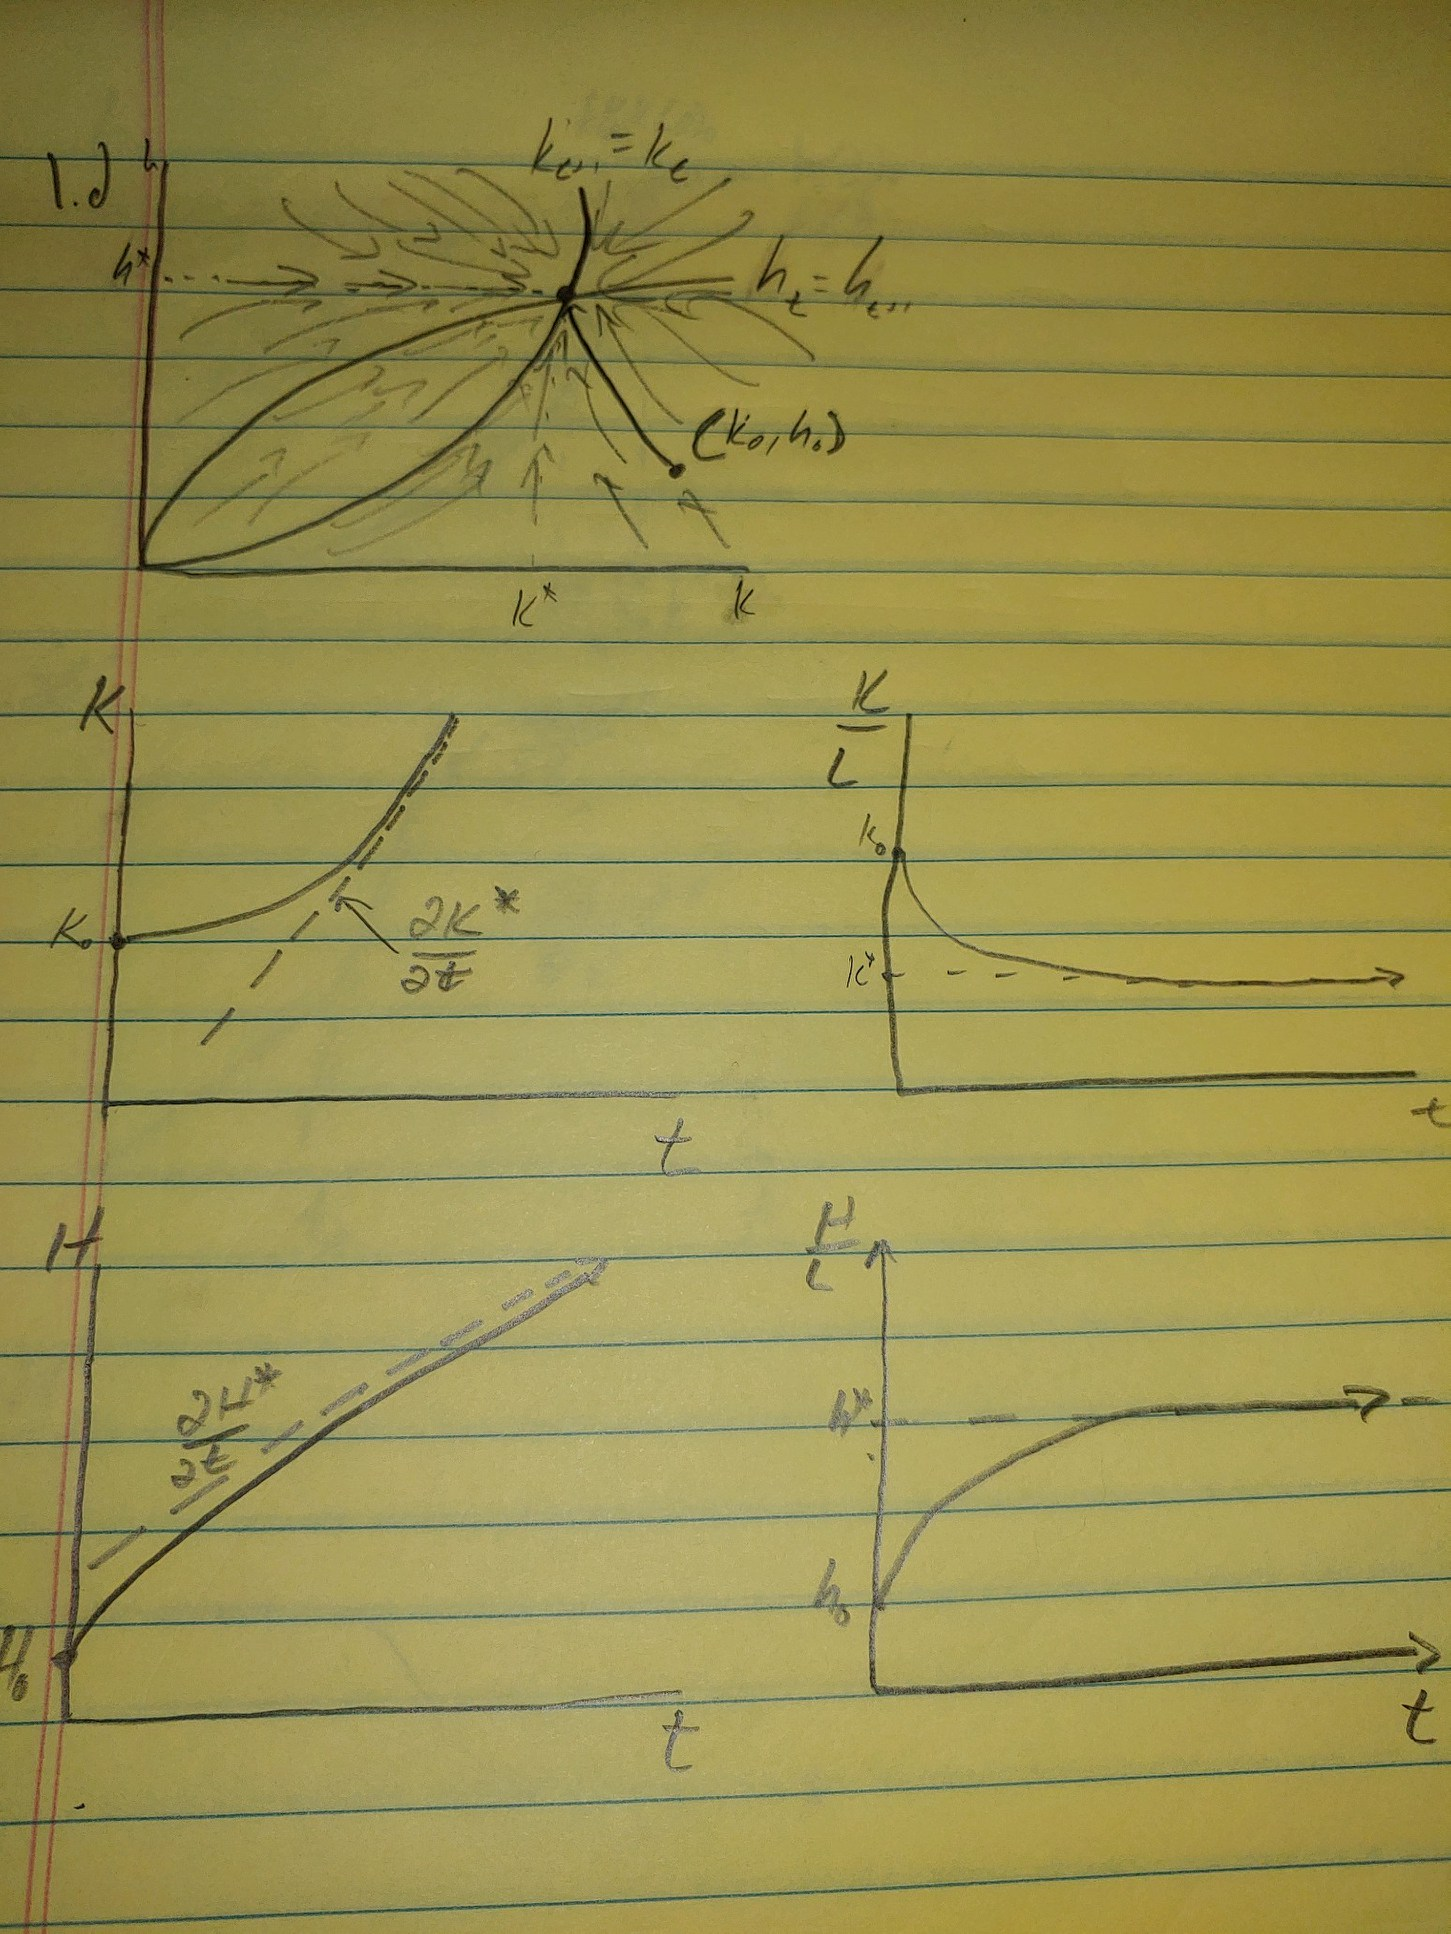
\includegraphics[scale=.2]{graph1d.JPG}\\
      \centering
    \end{solution}
    \item Assume that the economy is in its steady state when suddenly there is permanent increase in the growth rate of population $n$. Use the phase diagram to analyze the immediate and long run change to the economy. Additionally, plot the path of total \textit{GPD} and \textit{GPD per capita} over time.
    \begin{solution}
      By looking back at the dynamics equations we derived above, we can see the effect of moving from $n_0$ to $n_\prime$ with $n_0 < n_\prime$ is
      \begin{eqnarray*}
        k_0 = (\frac{s_K}{\delta + n_0})^\frac{1}{1 - \alpha}h_t^\frac{\beta}{1 - \alpha} > (\frac{s_K}{\delta + n_\prime})^\frac{1}{1 - \alpha}h_t^\frac{\beta}{1 - \alpha} = k_\prime
      \end{eqnarray*}
      and
      \begin{eqnarray*}
        h_0 = (\frac{s_H}{n_0})^\frac{1}{1 - \beta}k_t^\frac{\alpha}{1 - \beta} > (\frac{s_H}{n_\prime})^\frac{1}{1 - \beta}k_t^\frac{\alpha}{1 - \beta} = h_\prime
      \end{eqnarray*}
      So our phase diagram behaves as shown below. For simplicity, we relabel the lines $k_{t+1} - k_t = 0 \equiv k(t)$ and $h_{t+1} - h_t = 0 \equiv h(t)$. Notice that moving from $n_0$ to $n_\prime$ at time $t_n$ moves the economy from the lines $k(t)_0$ to $k(t)_\prime$ and $h(t)_0$ to $h(t)_\prime$ with $k(t)_0 > k(t)_\prime$ and $h(t)_0 > h(t)_\prime$. This puts the economy on track to a a new steady state of $(k_\prime^*,h_\prime^*)$ where $k_\prime^* < k_0^*$ and $h_\prime^* < h_0^*$. Finally, the time plots of GDP and GDP per Capita show us that GDP still doesn't reach a steady state but does reach a new, higher, steady state rate of change $\frac{\partial GDP}{\partial t}^\prime$ and GDP per capita reaches a new steady state value of $gdp_\prime^* < gdp_0^*$\\
      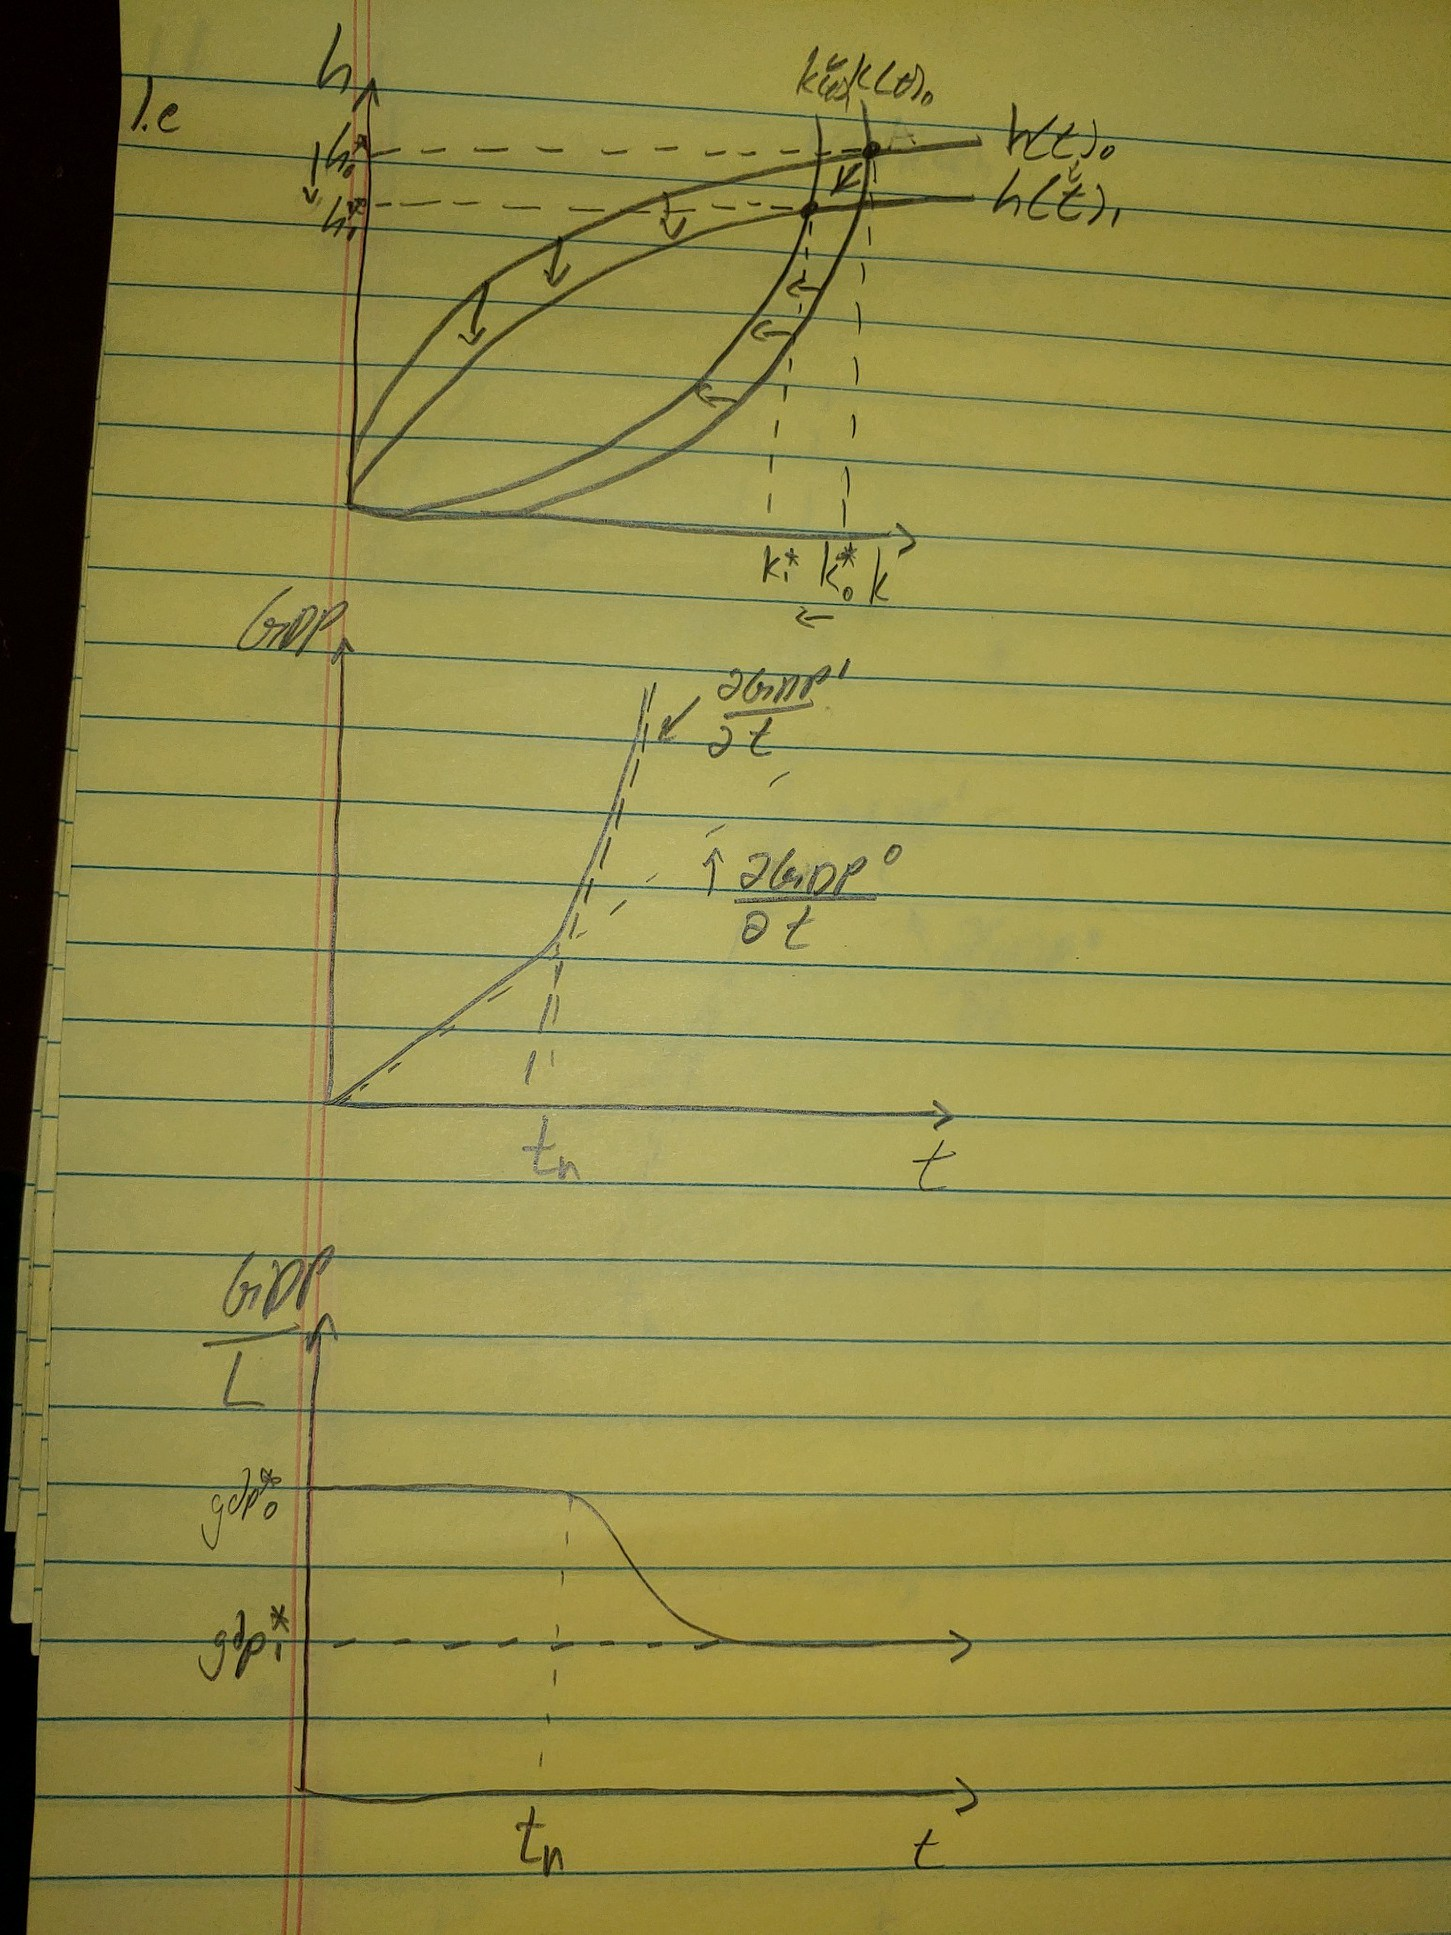
\includegraphics[scale=.2]{graph1e.JPG}\\
      \centering
    \end{solution}
    \item Instead, assume that the economy is in its steady state when suddenly there is permanent increase in the depreciation rate $\delta$. Use the phase diagram to analze the immediate and long run change to the economy. Additionally, plot the path of total \textit{GPD} and \textit{GPD per capita} over time.
    \begin{solution}
      Using the same terminology as above, the decrease in the value of $\delta$ from $\delta_0$ to $\delta_\prime$ where $\delta_0 > \delta_\prime$ does not affect the $h(t)$ line because human capital does not depreciate but it does shift $k(t)_0$ to $k(t)_\prime$ with $k(t)_0 < k(t)_\prime$ because
      \begin{eqnarray*}
        k_0 = (\frac{s_K}{\delta_0 + n})^\frac{1}{1 - \alpha}h_t^\frac{\beta}{1 - \alpha} < (\frac{s_K}{\delta_\prime + n})^\frac{1}{1 - \alpha}h_t^\frac{\beta}{1 - \alpha} = k_\prime
      \end{eqnarray*}
      This moves out steady state to $(k_\prime^*,h_\prime^*)$ where $k_\prime^* > k_0^*$ and $h_\prime^* > h_0^*$. The time plot of GDP behaves the same as it did before where it reaches a higher steady state rate of change but GDP per capita ends up moving to a higher steady state.\\
      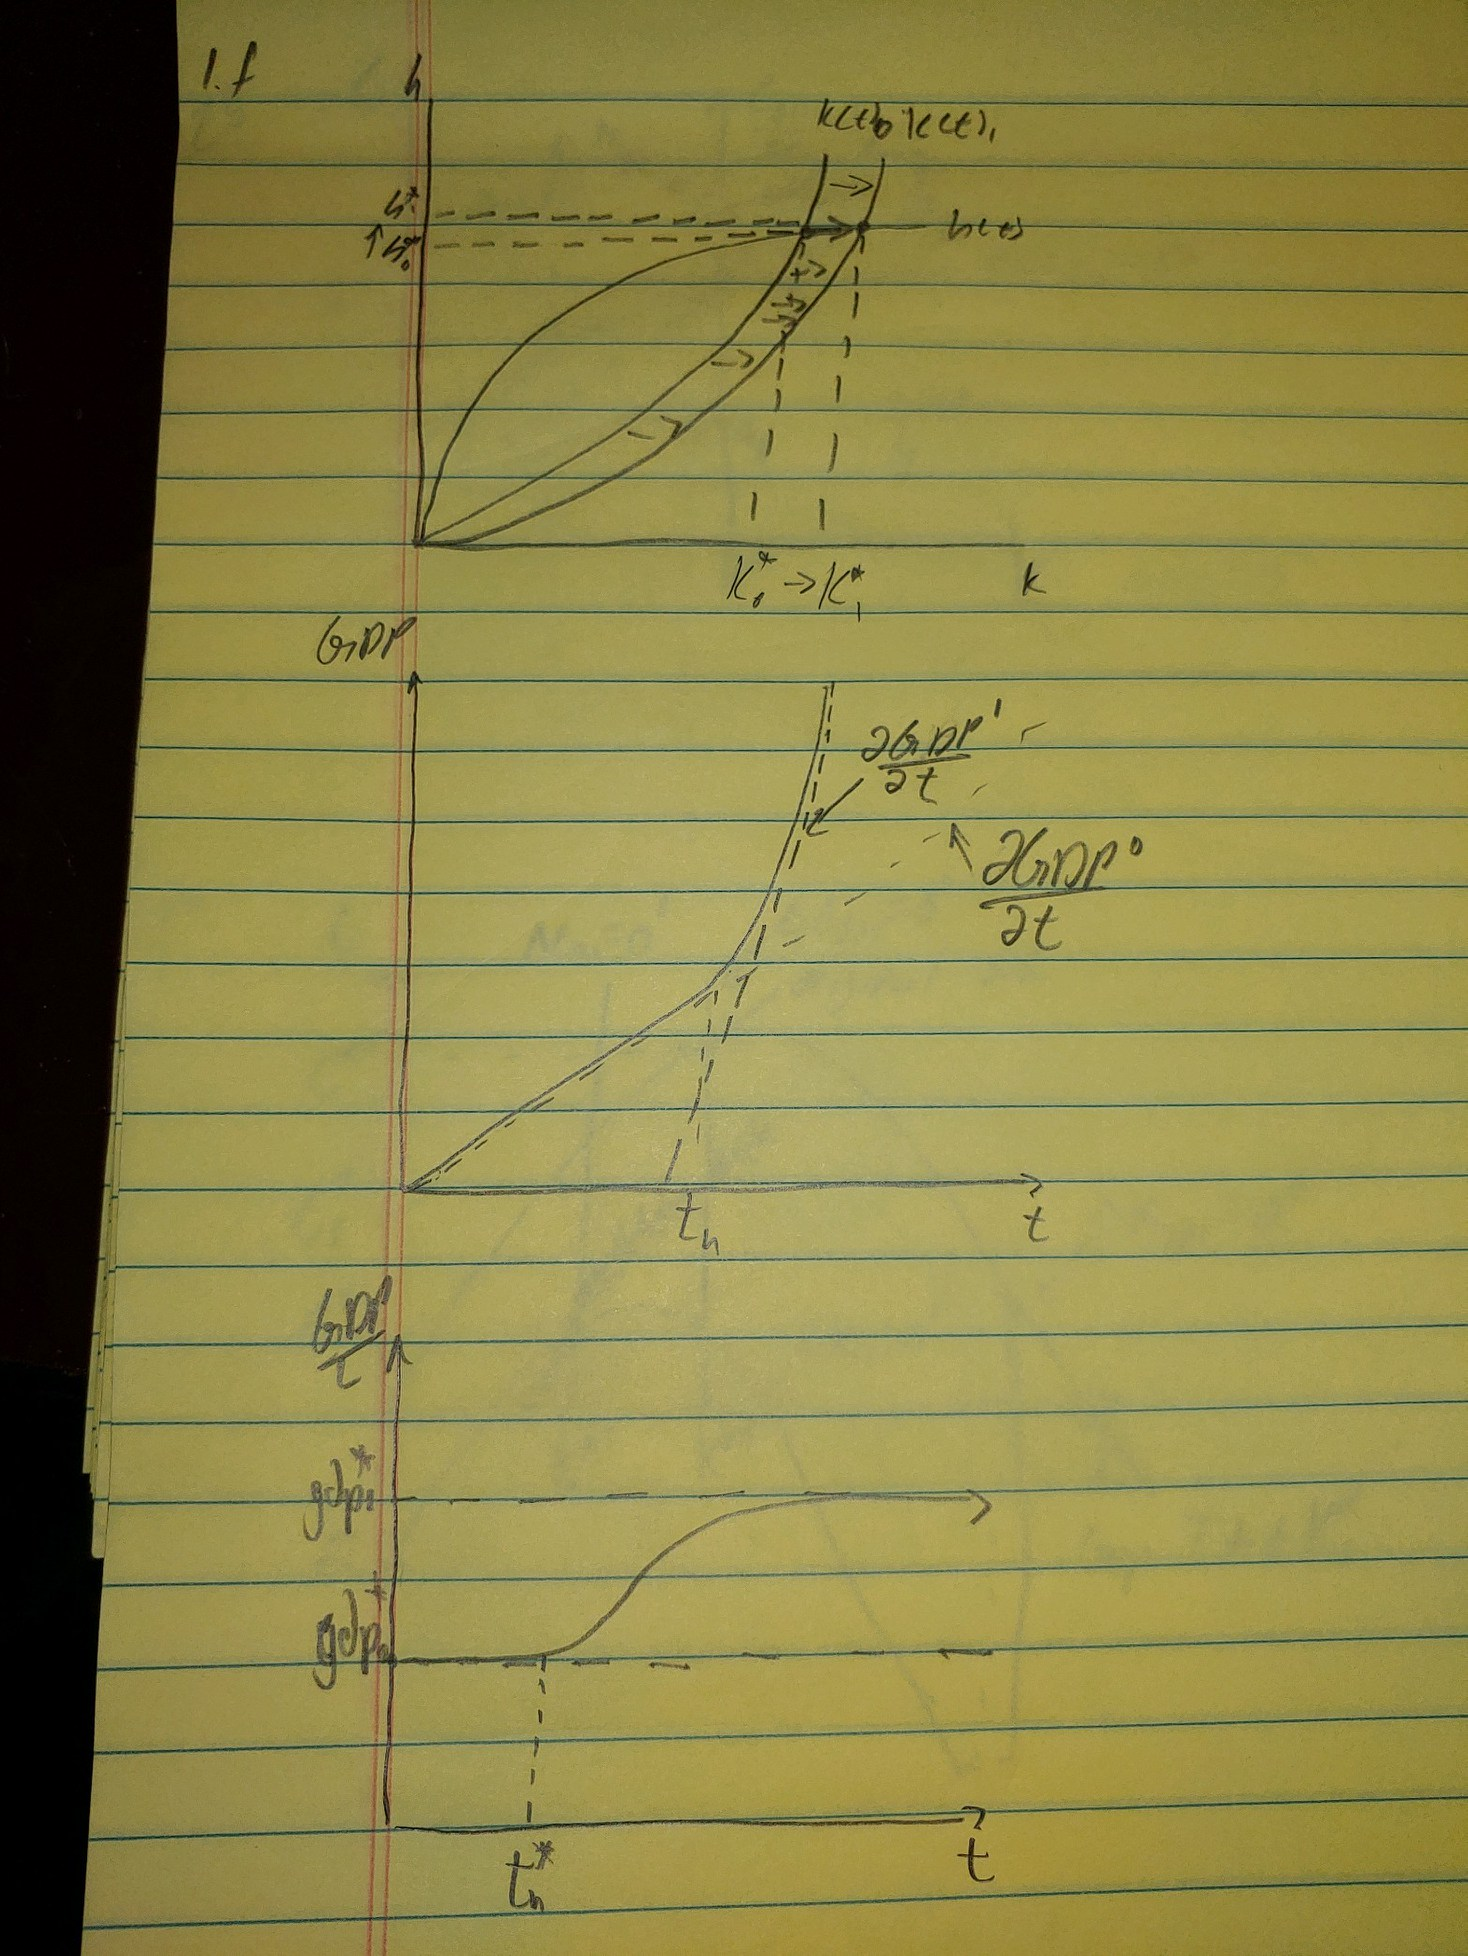
\includegraphics[scale=.2]{graph1f.JPG}\\
      \centering
    \end{solution}
  \end{enumerate}

  \item In the neoclassical growth model technology and population are constant and the government can impose two types of taxes on the household: a lump sum tax on household income or a proportional tax on output. That means that a household's budget constraint is
  \begin{eqnarray*}
    K_{s + 1} = (1 - \delta)K_s + (1 - \tau_s)K_s^\alpha - C_s - T_s
  \end{eqnarray*}
  where $T_s$ is the lump sum tax in year $s$ and $\tau$ is the proportional tax on output in year $s$ and everything else is as usual.
  \begin{enumerate}
    \item Write down the Euler equation for the household. Make sure you use appropriate time subscripts for each variable in the equation.
    \begin{solution}
      The household Euler equation is
      \begin{eqnarray*}
        u^\prime(C_s) = \beta(1 + (1 - \tau)F^\prime(K_{s+1}))u^\prime(C_{s+1})
      \end{eqnarray*}
    \end{solution}
    \item Suppose initially the economy is in steady state and there are no taxes ($\tau_s = T_s = 0 \; \forall s$). Draw the phase diagram and show the steady state.
    \begin{solution}
      We see from the phase diagram that the economy begins in at $(C^*,K^*)$ which is the steady state. We also see the "saddly path stable" nature of the phase space showing how different starting spots lead towards or away from the steady state as well.\\
      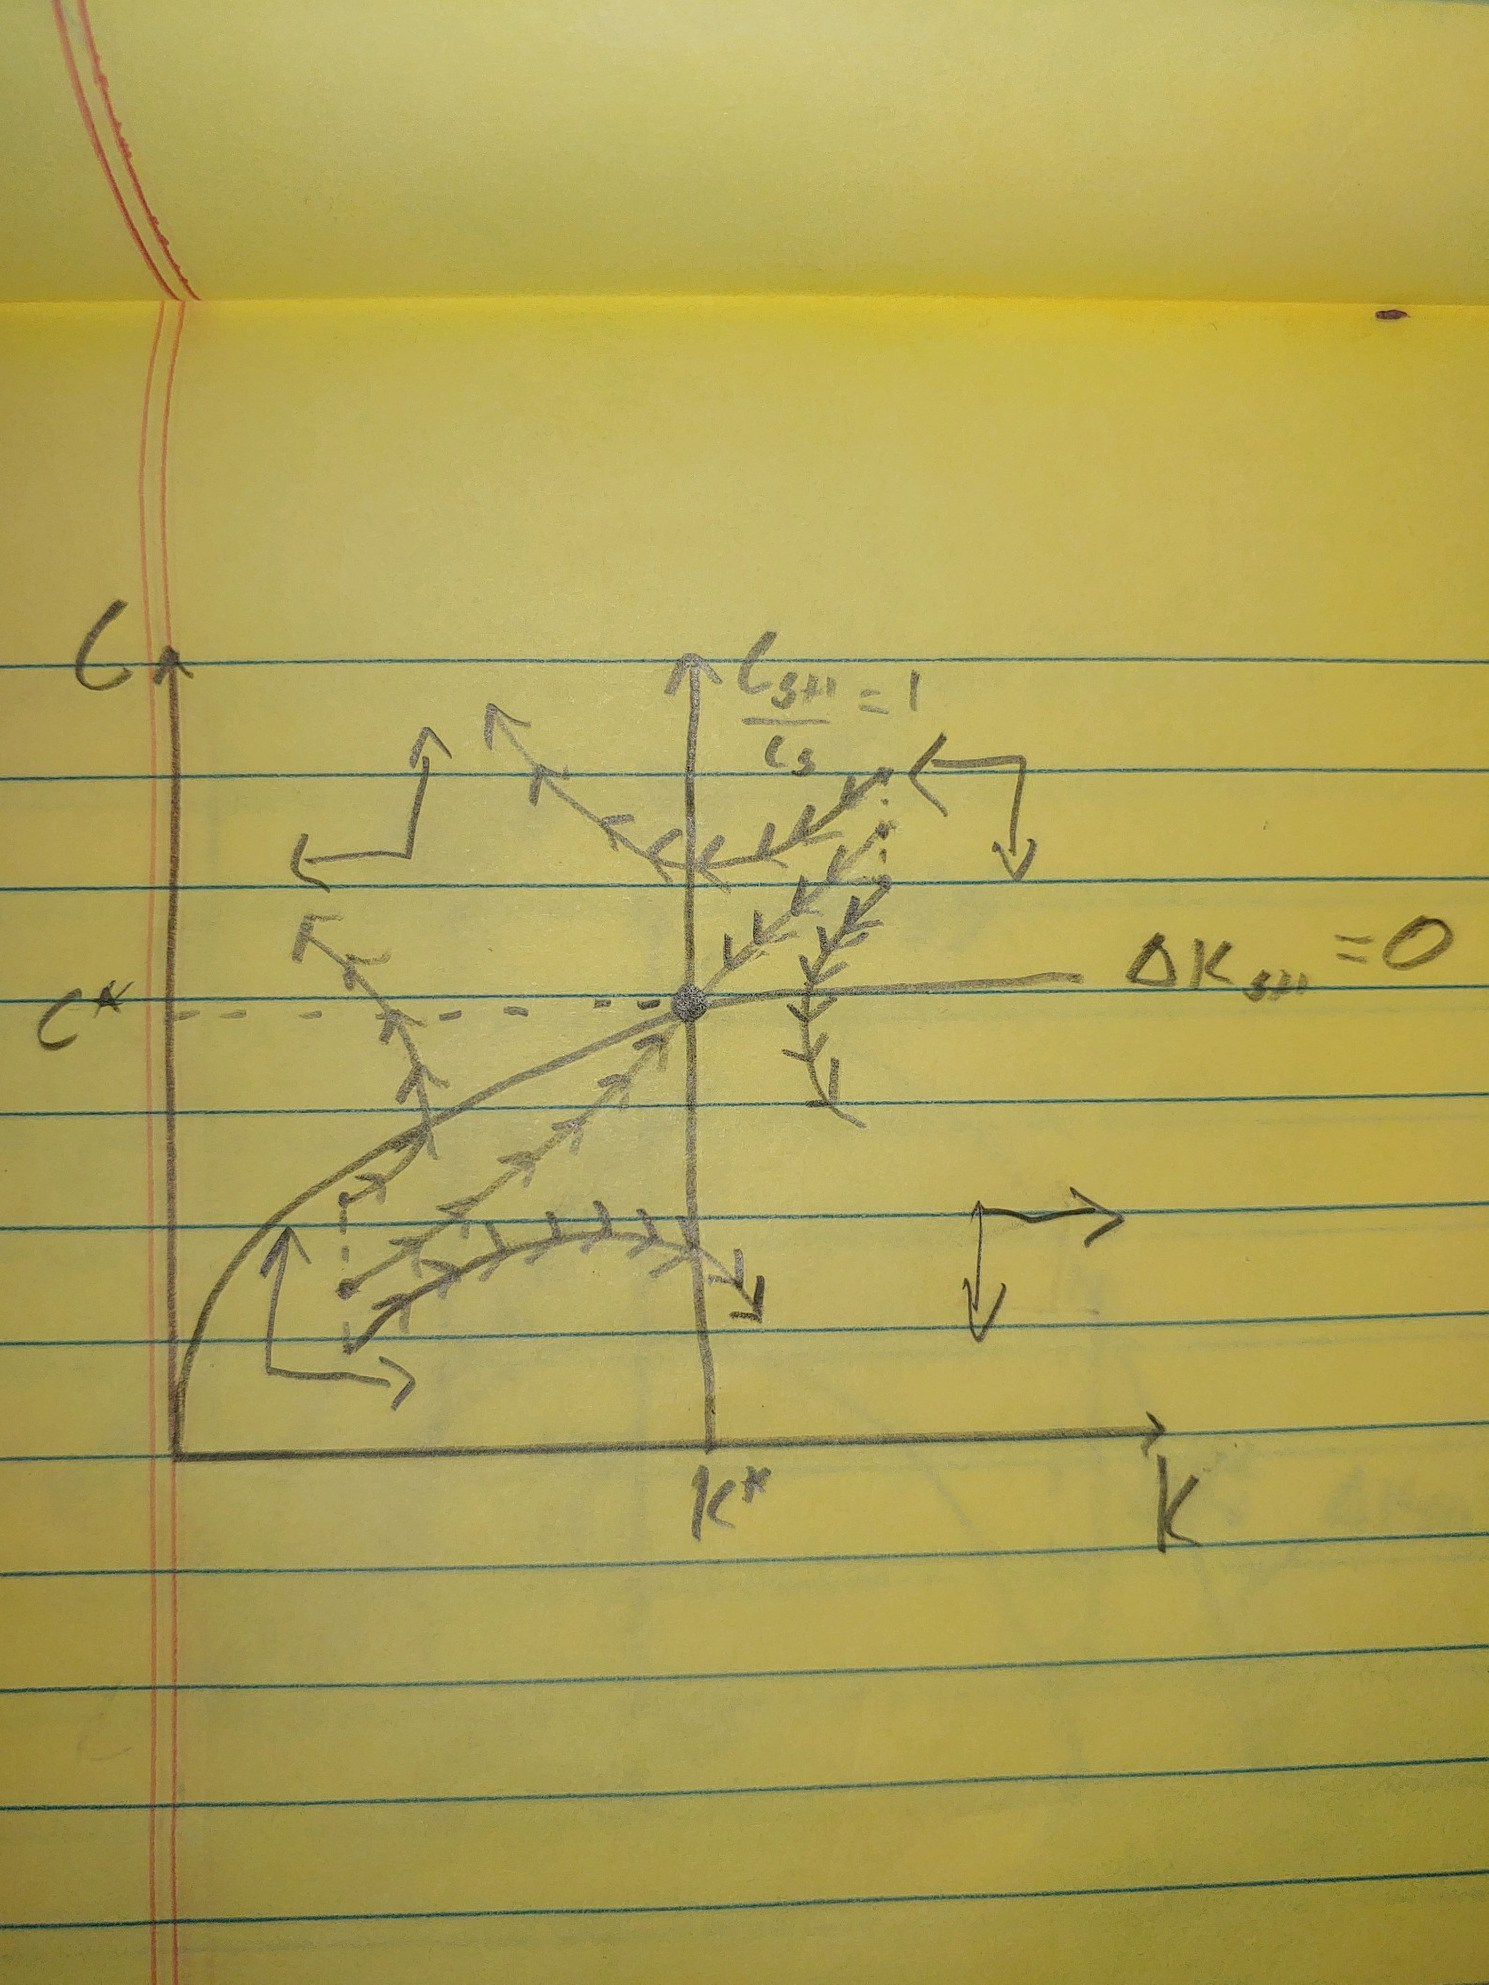
\includegraphics[scale=.2]{graph2b.JPG}\\
      \centering
    \end{solution}
    Seperately consider the following scenarios (each starting in the above steady state with no taxes).
    \item Starting with the economy in steady state, the government, unexpectedly and permanently, introduces \textbf{constant taxes} of both types, so that $\tau_s = \tau > 0$ and $T_s = T > 0$ from now on. Draw the phase diagram and show the steady state. Constrast it with the original one and show the dynamics of the economy as it moves to a new steady state (if there is a new steady state).
    \begin{solution}
      Increasing $T_s$ will cause a downward shift in the line representing $\Delta K_{s+1} = 0$ but will not shift the line representing $\frac{C_{s+1}}{C_s} = 1$. The increase in $\tau_s$ will shift the line representing $\frac{C_{s+1}}{C_s} = 1$ left and shift the the line representing $\Delta K_{s+1} = 0$ down. In order for the economy to reach the new steady state, consumption must immediately drop to to $C^\prime_s$ which puts the economy on the new stable arm and then eventually leads it to the new steady state.\\
      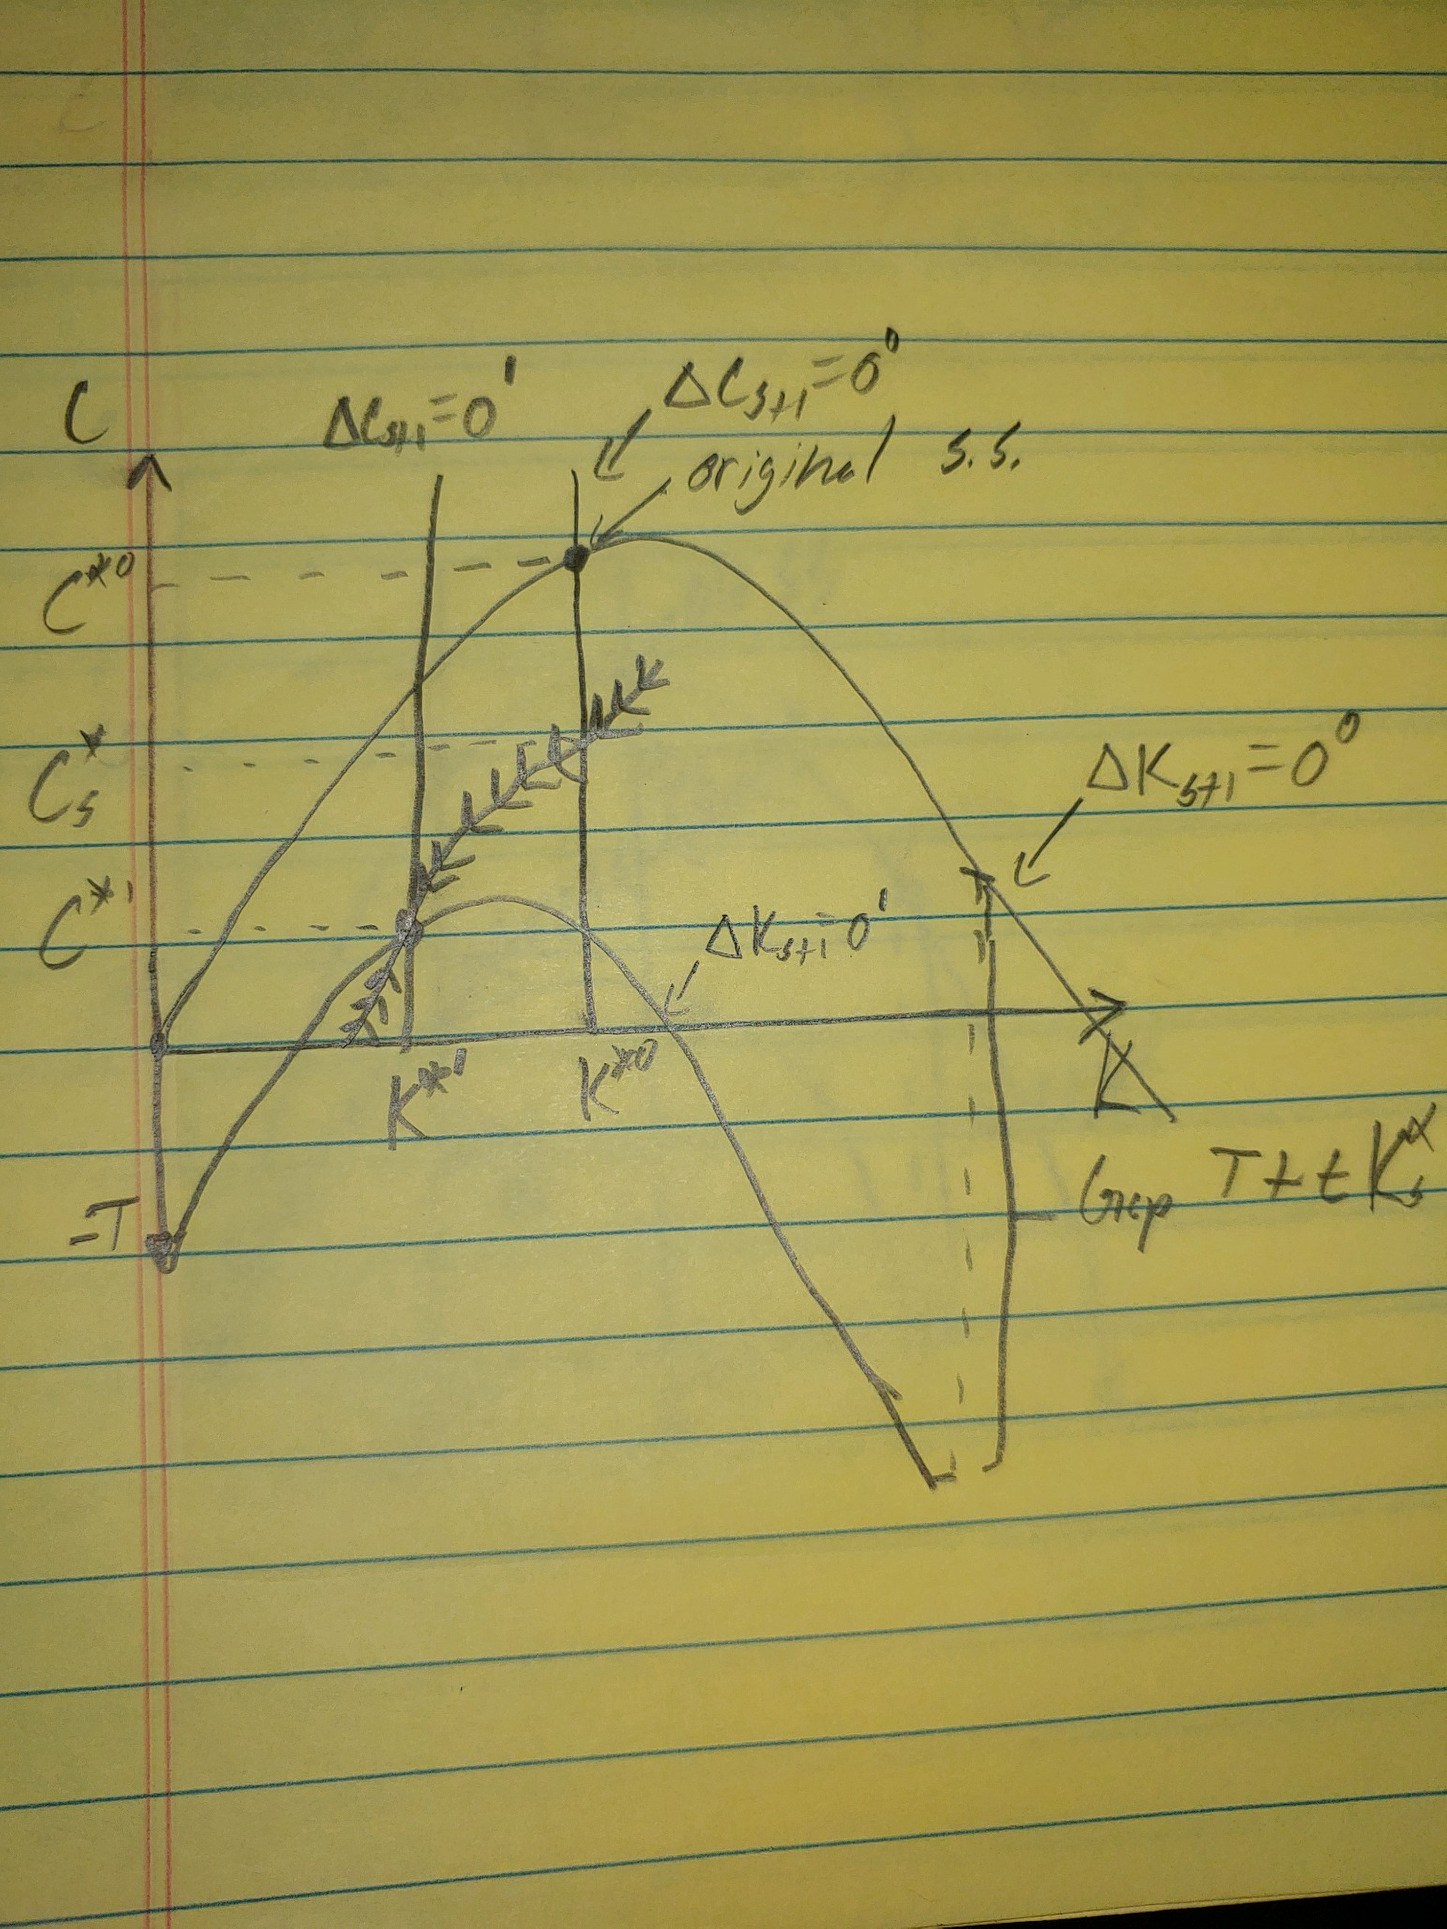
\includegraphics[scale=.2]{graph2c.JPG}\\
      \centering
    \end{solution}
    \item Starting with the economy in steady state, the government, unexpectedly and permanently, introduces \textbf{non-constant taxes} of both types. In this case, we are also told that the proportional tax $\tau$ is indeed constant, while the lump sum tax will be variable and given by $T_s = \tau K_s^\alpha$. Draw the phase diagram and show the steady state. Contrast it with the original one and show the dynamics of the economy as it moves to a new steady state (if there is a new steady state).
    \begin{solution}
      This new tax policy will have a similar affect to the one discussed in part (c) where the line representing $\Delta C_{s+1} = 0$ shifts to the left and $\Delta K_{s+1} = 0$ shifts down. However, because $T = \tau K_s^\alpha$, the gap between the original line for $\Delta K_{s+1} = 0$ and the new one will be $2\tau K_s^\alpha$. For the economy to reach the new steady state, again, consumption must immediatly fall to the new stable arm at $C^\prime_s$\\
      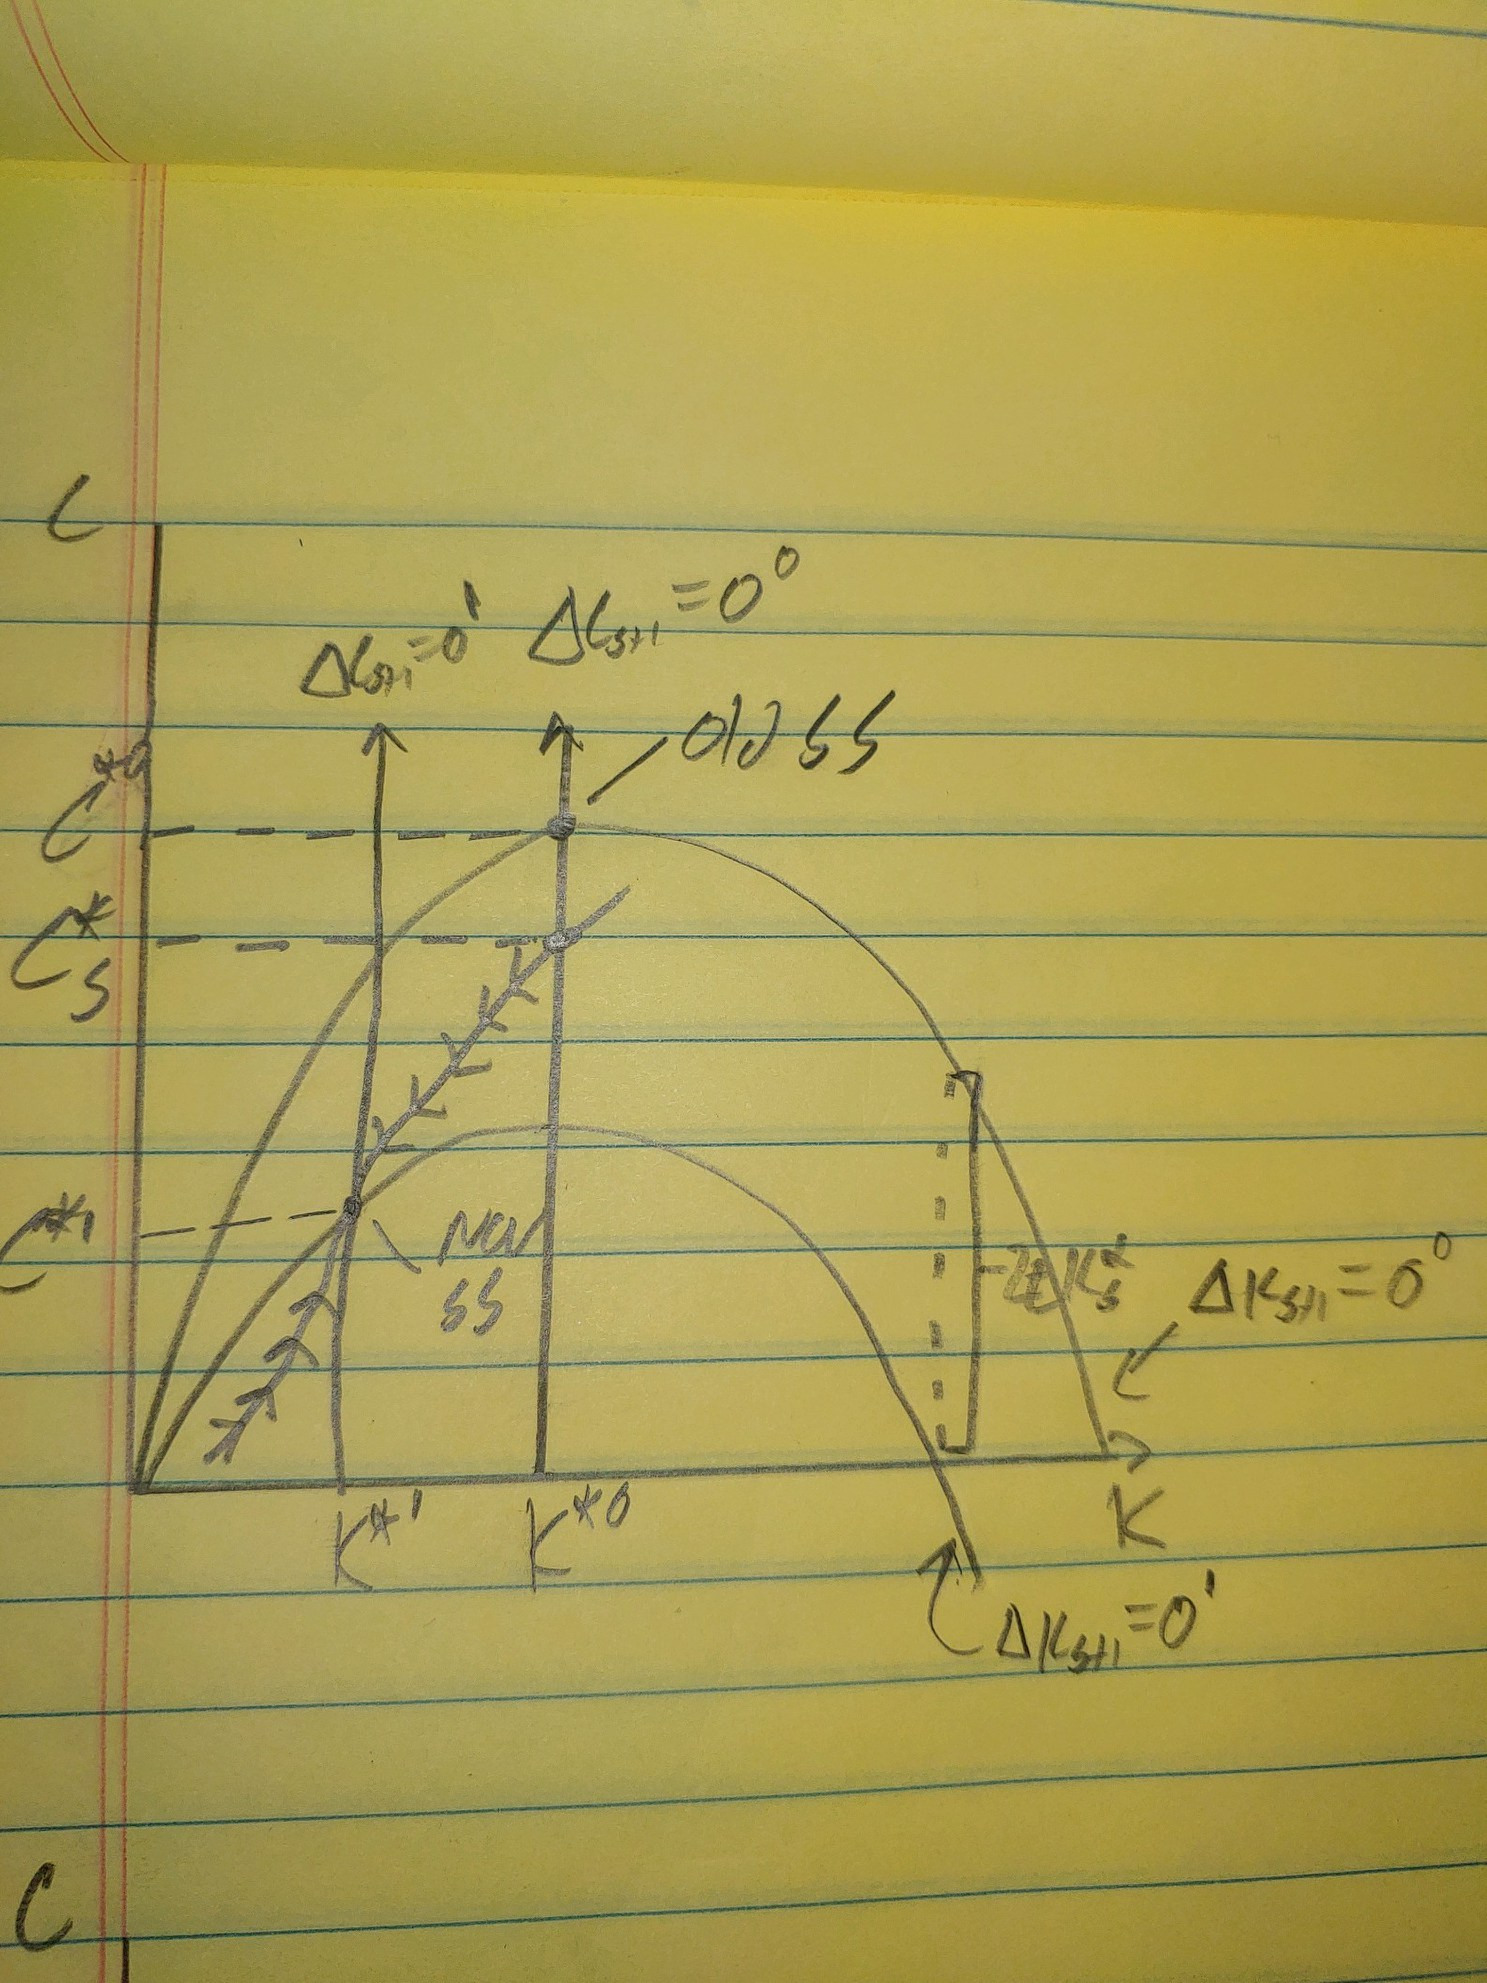
\includegraphics[scale=.2]{graph2d.JPG}\\
      \centering
    \end{solution}
    \item Same situation the same is in (d) above but now the change in tax policy is announced 5 years in advance (that is 5 years before the taxes are actually introduced). Draw the phase diagram and show the steady state. Contrast it with the original one and show the dynamics of the economy as it moves to a new steady state (if there is a new steady state). Also, carefully plot the time paths of capital and consumption, Make sure to explain when and why any changes occur.
    \begin{solution}
      The lines representing $\Delta K_{s+1} = 0$ and $\Delta C_{s+1} = 0$ will move the exact same way as they did in (d) but the economy's response will be different. In this case, consumption will immediately drop to the point $A$ and because the taxes have not been put into place yet, the system will still abide by the original dynamics. This moves the economy from $A$ to $B$ and at the moment the taxes begin and new the dynamics take effect. Because $B$ is on the new stable arm, the economy will then go to the new steady state.\\
      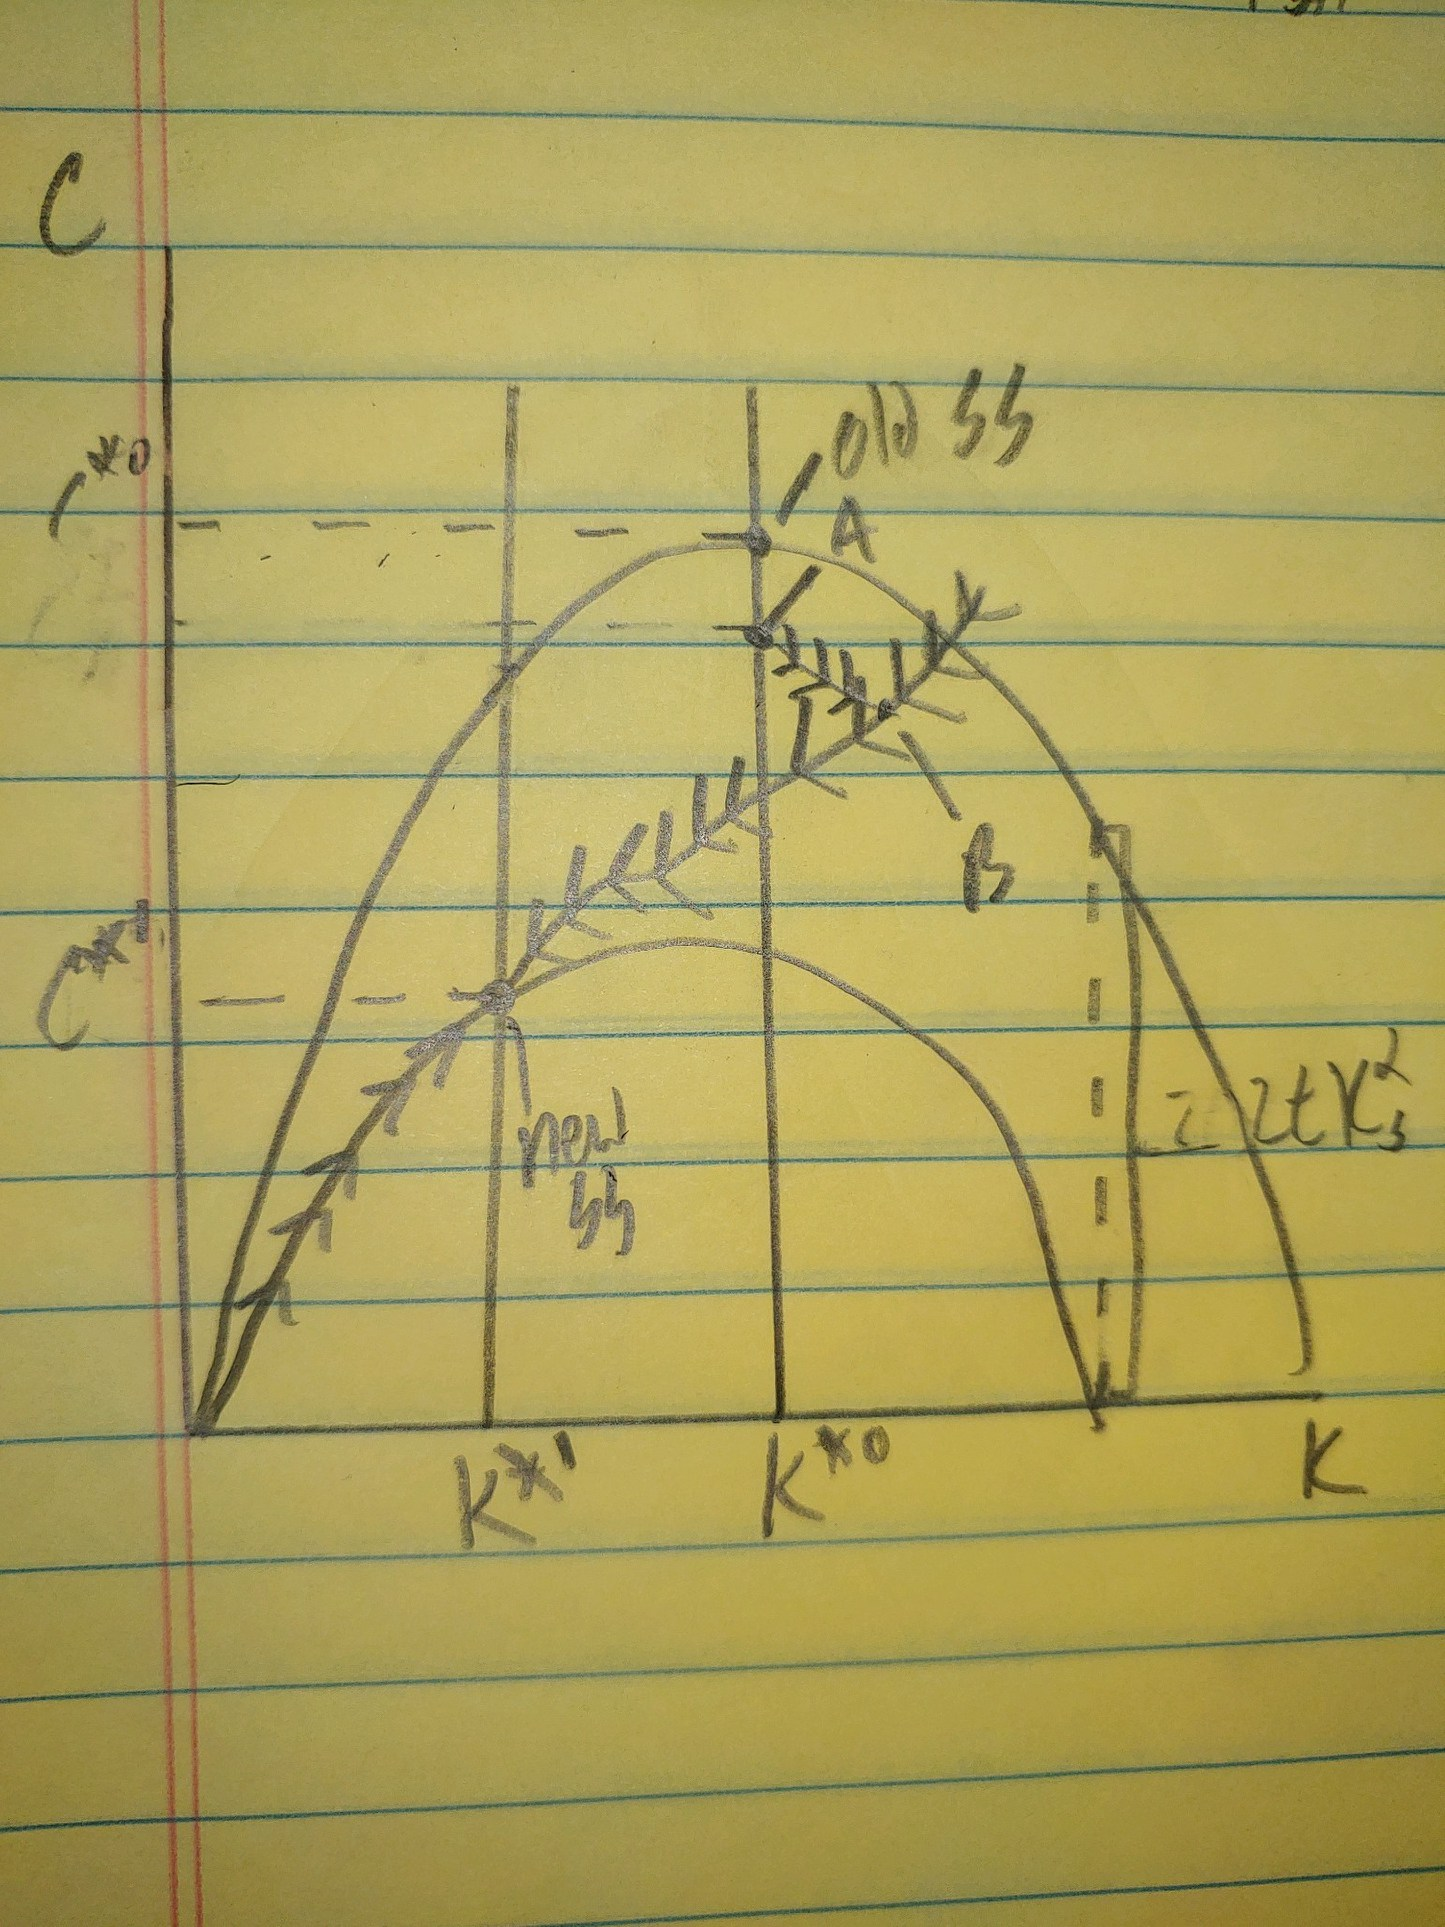
\includegraphics[scale=.2]{graph2e.JPG}\\
      \centering
    \end{solution}
  \end{enumerate}
\end{enumerate}
\end{document}